\def\latexbokFontdir{../../fonts}
\def\latexbokFiguredir{../../examples}
\documentclass[../../a4.tex]{subfiles}
\begin{document}
\section{Grafik med \LaTeX}\label{sec:4}

\subsection{Vad är bra grafik?}
% Se #26 på bitbucket
\subsubsection{Almänna tips}
\subsubsection{Programspecifika tips}
\subsubsubsection*{Bra \Rlogo-figurer med \texttt{ggplot2}}
\label{sec:ggplot2}
Standardgrafiken i \Rlogo är överlag ganska bra när det gäller statistisk
analys, men bristande på andra områden. På många sätt är det dessutom svårt
att göra lite mer involverade saker som att ändra färger, sätta ordentliga
axlar, enheter och så vidare. \Rlogo-paketet \texttt{ggplot2}
skapades för att åtgärda detta, och skapar snyggare grafer på enklare sätt.

% Fler anledningar:
% * Makes doing the right thing easy, while keeping harder things possible.
% * ggplot2 is an intuitive library that is founded on a logical mapping between data and graphical elements, building plots up not by thinking in terms of dots on paper, but in terms of what the data means. Think about your data and what you want to communicate, not the mechanics of drawing.

Att installera och använda \texttt{ggplot2} är enkelt. Efter att ha installerat
paketet genom att köra kommandot \verb|install.packages("ggplot2")| i \Rlogo
använder man det genom att inkludera paketet och använda funktionen
\texttt{ggplot} i kombination med någon av paketets många plot-funktioner.
Man kan även kombinera olika grafer:
\begin{rcode}
require(ggplot2)
# Exempeldata
df <- data.frame(
+   trt = factor(c(1, 1, 2, 2)),
+   resp = c(1, 5, 3, 4), 
+   group = factor(c(1, 2, 1, 2)),
+   se = c(0.1, 0.3, 0.3, 0.2)
+) 
df2 <- df[c(1,3),] 
# Toppen/botten på errorbars
limits <- aes(ymax = resp + se, ymin=resp - se)
dodge <- position_dodge(width=0.9)
# Plotta!
p <- ggplot(df, aes(fill=group, y=resp, x=trt))
p + geom_bar(position=dodge) +
  + geom_errorbar(limits, position=dodge, width=0.25)
\end{rcode}

En mer utförlig referens över alla kommandon i \texttt{ggplot2} finns på internet%
\footnote{\url{http://had.co.nz/ggplot2/}}, och en grundlig genomgång ges av
\citeasnoun{Hadley09}.
% Att tänka på: ggplot2 
\subsubsubsection*{Bättre \MATLAB-figurer}
% ???

\subsection{Inkludera grafik}
\subsubsection{Paketet \pack{graphicx}}
\subsubsection{Rita med \PGFTikZ}
\subsubsection{Varför hamnar figuren fel?}

\subsection{Exportera grafik}
När man väl skapat sin grafik i det program man arbetar med och är nöjd
med denna måste man exportera den till ett format som kan användas med
\LaTeX. Använder man \pdfLaTeX (vilket man bör) så stöds formaten \JPEG,
\PNG och \PDF. Av dessa lämpar sig \JPEG bäst till fotografier, medan
\PNG och \PDF lämpar sig väl till figurer och grafer.
Generellt sett är \PDF att föredra då formatet är vektorbaserat och
därför kan skalas både upp och ner utan att man förlorar någon kvalitet.

Om möjligheten finns är det bästa dock att exportera sina figurer som
\PGFTikZ-kod, vilket innebär att \LaTeX{} kommer att rendera dem och att
man därför har något större frihet när det gäller finjustering av figuren
i efterhand, och även att axlar och dylikt typsätts på samma sätt som
dokumentets brödtext vilket ger ett enhetligt intryck.

Det finns många (matematiska) programvaror, och det är orimligt att
inkludera instruktioner till alla i detta kapitel. Jag har därför valt
att beskriva hur man enklast exporterar figurer som \PGFTikZ-kod eller
i \PDF-format (i nödfall \PNG) från fyra vanliga programvaror:
\Rlogo, \MATLAB, \Mathematica och \gnuplot.

\subsubsection{Exportera i \PGFTikZ-format}
\PGFTikZ brukar inte vara ett format som normalt stöds av kommersiella
(eller fria) programvaror, och därför är funktionen ofta implementerad
som någon form av tillägg. Lyckligtvis brukar dessa vara öppna och fria
att använda för vem som helst.

\subsubsubsection*{Från \Rlogo med \texttt{tikzDevice}}
\Rlogo-paketet \texttt{tikzDevice} \cite{Sharpsteen12} gör det möjligt
att i \Rlogo exportera figurer som \PGFTikZ-kod. Det kan som många andra
\Rlogo-paket hittas på CRAN och installeras enklast genom att köra
\Rlogo-kommandot \verb|install.packages("tikzDevice")|. Man använder
sedan kommandot \texttt{tikz} för att berätta för \Rlogo att grafiken
ska skrivas som \PGFTikZ-kod, och filen som skapas kan sedan inkluderas
i \LaTeX-dokument med kommandot \cmd{input}.
Exempel~\vref{ex:tikzdevice} visar resultatet av detta.

\begin{kod}[tbp]
	\centering
	\begin{minipage}{\textwidth}
		\centering
		% Created by tikzDevice version 0.6.2-80-b0c08dc on 2012-07-31 03:25:08
% !TEX encoding = UTF-8 Unicode
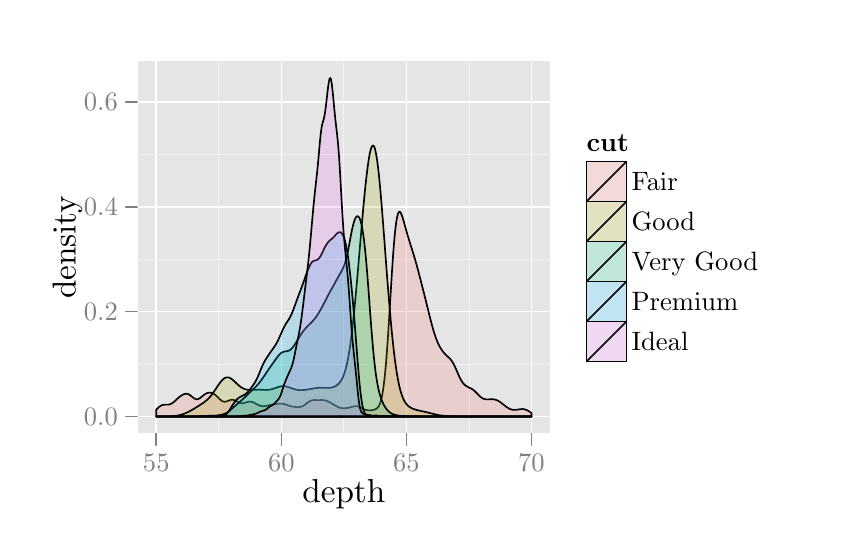
\begin{tikzpicture}[x=1pt,y=1pt]
\definecolor[named]{fillColor}{rgb}{1.00,1.00,1.00}
\path[use as bounding box,fill=fillColor,fill opacity=0.00] (0,0) rectangle (289.08,180.67);
\begin{scope}
\path[clip] (  0.00,  0.00) rectangle (289.08,180.67);
\definecolor[named]{fillColor}{rgb}{1.00,1.00,1.00}

\path[fill=fillColor] ( -0.00,  0.00) rectangle (289.08,180.68);
\end{scope}
\begin{scope}
\path[clip] (  0.00,  0.00) rectangle (289.08,180.67);
\definecolor[named]{drawColor}{rgb}{0.50,0.50,0.50}

\node[text=drawColor,anchor=base east,inner sep=0pt, outer sep=0pt, scale=  0.96] at ( 32.57, 36.85) {0.0};

\node[text=drawColor,anchor=base east,inner sep=0pt, outer sep=0pt, scale=  0.96] at ( 32.57, 74.75) {0.2};

\node[text=drawColor,anchor=base east,inner sep=0pt, outer sep=0pt, scale=  0.96] at ( 32.57,112.66) {0.4};

\node[text=drawColor,anchor=base east,inner sep=0pt, outer sep=0pt, scale=  0.96] at ( 32.57,150.57) {0.6};
\end{scope}
\begin{scope}
\path[clip] (  0.00,  0.00) rectangle (289.08,180.67);
\definecolor[named]{drawColor}{rgb}{0.50,0.50,0.50}

\path[draw=drawColor,line width= 0.6pt,line join=round,line cap=round] ( 35.42, 40.15) -- ( 39.69, 40.15);

\path[draw=drawColor,line width= 0.6pt,line join=round,line cap=round] ( 35.42, 78.06) -- ( 39.69, 78.06);

\path[draw=drawColor,line width= 0.6pt,line join=round,line cap=round] ( 35.42,115.97) -- ( 39.69,115.97);

\path[draw=drawColor,line width= 0.6pt,line join=round,line cap=round] ( 35.42,153.87) -- ( 39.69,153.87);
\end{scope}
\begin{scope}
\path[clip] ( 39.69, 34.03) rectangle (188.82,168.63);
\definecolor[named]{fillColor}{rgb}{0.90,0.90,0.90}

\path[fill=fillColor] ( 39.69, 34.03) rectangle (188.82,168.63);
\definecolor[named]{drawColor}{rgb}{0.95,0.95,0.95}

\path[draw=drawColor,line width= 0.3pt,line join=round,line cap=round] ( 39.69, 59.11) --
	(188.82, 59.11);

\path[draw=drawColor,line width= 0.3pt,line join=round,line cap=round] ( 39.69, 97.01) --
	(188.82, 97.01);

\path[draw=drawColor,line width= 0.3pt,line join=round,line cap=round] ( 39.69,134.92) --
	(188.82,134.92);

\path[draw=drawColor,line width= 0.3pt,line join=round,line cap=round] ( 69.06, 34.03) --
	( 69.06,168.63);

\path[draw=drawColor,line width= 0.3pt,line join=round,line cap=round] (114.25, 34.03) --
	(114.25,168.63);

\path[draw=drawColor,line width= 0.3pt,line join=round,line cap=round] (159.45, 34.03) --
	(159.45,168.63);
\definecolor[named]{drawColor}{rgb}{1.00,1.00,1.00}

\path[draw=drawColor,line width= 0.6pt,line join=round,line cap=round] ( 39.69, 40.15) --
	(188.82, 40.15);

\path[draw=drawColor,line width= 0.6pt,line join=round,line cap=round] ( 39.69, 78.06) --
	(188.82, 78.06);

\path[draw=drawColor,line width= 0.6pt,line join=round,line cap=round] ( 39.69,115.97) --
	(188.82,115.97);

\path[draw=drawColor,line width= 0.6pt,line join=round,line cap=round] ( 39.69,153.87) --
	(188.82,153.87);

\path[draw=drawColor,line width= 0.6pt,line join=round,line cap=round] ( 46.47, 34.03) --
	( 46.47,168.63);

\path[draw=drawColor,line width= 0.6pt,line join=round,line cap=round] ( 91.66, 34.03) --
	( 91.66,168.63);

\path[draw=drawColor,line width= 0.6pt,line join=round,line cap=round] (136.85, 34.03) --
	(136.85,168.63);

\path[draw=drawColor,line width= 0.6pt,line join=round,line cap=round] (182.04, 34.03) --
	(182.04,168.63);
\definecolor[named]{drawColor}{rgb}{0.00,0.00,0.00}
\definecolor[named]{fillColor}{rgb}{0.97,0.46,0.43}

\path[draw=drawColor,line width= 0.6pt,line join=round,line cap=round,fill=fillColor,fill opacity=0.20] ( 46.47, 42.65) --
	( 46.73, 42.92) --
	( 47.00, 43.18) --
	( 47.26, 43.42) --
	( 47.53, 43.65) --
	( 47.79, 43.85) --
	( 48.06, 44.02) --
	( 48.32, 44.16) --
	( 48.59, 44.27) --
	( 48.85, 44.35) --
	( 49.12, 44.40) --
	( 49.38, 44.43) --
	( 49.65, 44.45) --
	( 49.91, 44.45) --
	( 50.18, 44.45) --
	( 50.45, 44.45) --
	( 50.71, 44.46) --
	( 50.98, 44.49) --
	( 51.24, 44.55) --
	( 51.51, 44.62) --
	( 51.77, 44.73) --
	( 52.04, 44.86) --
	( 52.30, 45.03) --
	( 52.57, 45.22) --
	( 52.83, 45.43) --
	( 53.10, 45.66) --
	( 53.36, 45.90) --
	( 53.63, 46.15) --
	( 53.89, 46.41) --
	( 54.16, 46.65) --
	( 54.42, 46.89) --
	( 54.69, 47.12) --
	( 54.96, 47.34) --
	( 55.22, 47.54) --
	( 55.49, 47.72) --
	( 55.75, 47.89) --
	( 56.02, 48.03) --
	( 56.28, 48.15) --
	( 56.55, 48.25) --
	( 56.81, 48.33) --
	( 57.08, 48.37) --
	( 57.34, 48.38) --
	( 57.61, 48.35) --
	( 57.87, 48.29) --
	( 58.14, 48.18) --
	( 58.40, 48.04) --
	( 58.67, 47.87) --
	( 58.94, 47.67) --
	( 59.20, 47.46) --
	( 59.47, 47.24) --
	( 59.73, 47.03) --
	( 60.00, 46.84) --
	( 60.26, 46.67) --
	( 60.53, 46.54) --
	( 60.79, 46.45) --
	( 61.06, 46.41) --
	( 61.32, 46.42) --
	( 61.59, 46.48) --
	( 61.85, 46.59) --
	( 62.12, 46.73) --
	( 62.38, 46.91) --
	( 62.65, 47.11) --
	( 62.91, 47.33) --
	( 63.18, 47.55) --
	( 63.45, 47.77) --
	( 63.71, 47.98) --
	( 63.98, 48.17) --
	( 64.24, 48.34) --
	( 64.51, 48.48) --
	( 64.77, 48.60) --
	( 65.04, 48.69) --
	( 65.30, 48.75) --
	( 65.57, 48.78) --
	( 65.83, 48.78) --
	( 66.10, 48.76) --
	( 66.36, 48.71) --
	( 66.63, 48.63) --
	( 66.89, 48.53) --
	( 67.16, 48.40) --
	( 67.43, 48.24) --
	( 67.69, 48.05) --
	( 67.96, 47.84) --
	( 68.22, 47.60) --
	( 68.49, 47.35) --
	( 68.75, 47.08) --
	( 69.02, 46.81) --
	( 69.28, 46.55) --
	( 69.55, 46.30) --
	( 69.81, 46.08) --
	( 70.08, 45.88) --
	( 70.34, 45.72) --
	( 70.61, 45.60) --
	( 70.87, 45.53) --
	( 71.14, 45.50) --
	( 71.41, 45.52) --
	( 71.67, 45.56) --
	( 71.94, 45.64) --
	( 72.20, 45.73) --
	( 72.47, 45.84) --
	( 72.73, 45.94) --
	( 73.00, 46.04) --
	( 73.26, 46.12) --
	( 73.53, 46.18) --
	( 73.79, 46.20) --
	( 74.06, 46.20) --
	( 74.32, 46.16) --
	( 74.59, 46.09) --
	( 74.85, 45.99) --
	( 75.12, 45.86) --
	( 75.38, 45.73) --
	( 75.65, 45.58) --
	( 75.92, 45.43) --
	( 76.18, 45.29) --
	( 76.45, 45.17) --
	( 76.71, 45.07) --
	( 76.98, 45.00) --
	( 77.24, 44.95) --
	( 77.51, 44.94) --
	( 77.77, 44.95) --
	( 78.04, 45.00) --
	( 78.30, 45.06) --
	( 78.57, 45.14) --
	( 78.83, 45.23) --
	( 79.10, 45.32) --
	( 79.36, 45.40) --
	( 79.63, 45.47) --
	( 79.90, 45.52) --
	( 80.16, 45.54) --
	( 80.43, 45.54) --
	( 80.69, 45.51) --
	( 80.96, 45.45) --
	( 81.22, 45.37) --
	( 81.49, 45.26) --
	( 81.75, 45.14) --
	( 82.02, 45.00) --
	( 82.28, 44.86) --
	( 82.55, 44.72) --
	( 82.81, 44.58) --
	( 83.08, 44.44) --
	( 83.34, 44.31) --
	( 83.61, 44.20) --
	( 83.87, 44.11) --
	( 84.14, 44.03) --
	( 84.41, 43.97) --
	( 84.67, 43.92) --
	( 84.94, 43.90) --
	( 85.20, 43.89) --
	( 85.47, 43.91) --
	( 85.73, 43.93) --
	( 86.00, 43.97) --
	( 86.26, 44.02) --
	( 86.53, 44.08) --
	( 86.79, 44.14) --
	( 87.06, 44.21) --
	( 87.32, 44.27) --
	( 87.59, 44.33) --
	( 87.85, 44.38) --
	( 88.12, 44.43) --
	( 88.39, 44.48) --
	( 88.65, 44.52) --
	( 88.92, 44.56) --
	( 89.18, 44.59) --
	( 89.45, 44.63) --
	( 89.71, 44.67) --
	( 89.98, 44.70) --
	( 90.24, 44.74) --
	( 90.51, 44.77) --
	( 90.77, 44.80) --
	( 91.04, 44.82) --
	( 91.30, 44.83) --
	( 91.57, 44.83) --
	( 91.83, 44.82) --
	( 92.10, 44.78) --
	( 92.36, 44.74) --
	( 92.63, 44.68) --
	( 92.90, 44.60) --
	( 93.16, 44.52) --
	( 93.43, 44.43) --
	( 93.69, 44.33) --
	( 93.96, 44.23) --
	( 94.22, 44.14) --
	( 94.49, 44.06) --
	( 94.75, 43.98) --
	( 95.02, 43.90) --
	( 95.28, 43.84) --
	( 95.55, 43.79) --
	( 95.81, 43.74) --
	( 96.08, 43.70) --
	( 96.34, 43.66) --
	( 96.61, 43.63) --
	( 96.88, 43.60) --
	( 97.14, 43.58) --
	( 97.41, 43.56) --
	( 97.67, 43.56) --
	( 97.94, 43.57) --
	( 98.20, 43.59) --
	( 98.47, 43.63) --
	( 98.73, 43.69) --
	( 99.00, 43.78) --
	( 99.26, 43.89) --
	( 99.53, 44.03) --
	( 99.79, 44.19) --
	(100.06, 44.36) --
	(100.32, 44.55) --
	(100.59, 44.75) --
	(100.86, 44.96) --
	(101.12, 45.16) --
	(101.39, 45.35) --
	(101.65, 45.52) --
	(101.92, 45.68) --
	(102.18, 45.80) --
	(102.45, 45.91) --
	(102.71, 45.99) --
	(102.98, 46.04) --
	(103.24, 46.08) --
	(103.51, 46.10) --
	(103.77, 46.10) --
	(104.04, 46.10) --
	(104.30, 46.10) --
	(104.57, 46.09) --
	(104.83, 46.09) --
	(105.10, 46.09) --
	(105.37, 46.09) --
	(105.63, 46.10) --
	(105.90, 46.11) --
	(106.16, 46.11) --
	(106.43, 46.11) --
	(106.69, 46.10) --
	(106.96, 46.07) --
	(107.22, 46.03) --
	(107.49, 45.98) --
	(107.75, 45.92) --
	(108.02, 45.83) --
	(108.28, 45.74) --
	(108.55, 45.63) --
	(108.81, 45.50) --
	(109.08, 45.37) --
	(109.35, 45.22) --
	(109.61, 45.07) --
	(109.88, 44.91) --
	(110.14, 44.74) --
	(110.41, 44.57) --
	(110.67, 44.40) --
	(110.94, 44.24) --
	(111.20, 44.08) --
	(111.47, 43.92) --
	(111.73, 43.78) --
	(112.00, 43.65) --
	(112.26, 43.53) --
	(112.53, 43.43) --
	(112.79, 43.35) --
	(113.06, 43.28) --
	(113.32, 43.23) --
	(113.59, 43.19) --
	(113.86, 43.17) --
	(114.12, 43.16) --
	(114.39, 43.16) --
	(114.65, 43.17) --
	(114.92, 43.19) --
	(115.18, 43.22) --
	(115.45, 43.26) --
	(115.71, 43.30) --
	(115.98, 43.35) --
	(116.24, 43.41) --
	(116.51, 43.47) --
	(116.77, 43.54) --
	(117.04, 43.62) --
	(117.30, 43.69) --
	(117.57, 43.76) --
	(117.84, 43.82) --
	(118.10, 43.87) --
	(118.37, 43.90) --
	(118.63, 43.91) --
	(118.90, 43.90) --
	(119.16, 43.86) --
	(119.43, 43.80) --
	(119.69, 43.71) --
	(119.96, 43.60) --
	(120.22, 43.48) --
	(120.49, 43.35) --
	(120.75, 43.21) --
	(121.02, 43.07) --
	(121.28, 42.93) --
	(121.55, 42.81) --
	(121.81, 42.69) --
	(122.08, 42.60) --
	(122.35, 42.52) --
	(122.61, 42.46) --
	(122.88, 42.42) --
	(123.14, 42.39) --
	(123.41, 42.38) --
	(123.67, 42.38) --
	(123.94, 42.39) --
	(124.20, 42.42) --
	(124.47, 42.45) --
	(124.73, 42.50) --
	(125.00, 42.56) --
	(125.26, 42.64) --
	(125.53, 42.74) --
	(125.79, 42.86) --
	(126.06, 43.03) --
	(126.33, 43.25) --
	(126.59, 43.54) --
	(126.86, 43.92) --
	(127.12, 44.41) --
	(127.39, 45.08) --
	(127.65, 45.93) --
	(127.92, 47.01) --
	(128.18, 48.34) --
	(128.45, 49.96) --
	(128.71, 51.90) --
	(128.98, 54.18) --
	(129.24, 56.81) --
	(129.51, 59.81) --
	(129.77, 63.17) --
	(130.04, 66.88) --
	(130.31, 70.86) --
	(130.57, 75.05) --
	(130.84, 79.37) --
	(131.10, 83.76) --
	(131.37, 88.11) --
	(131.63, 92.35) --
	(131.90, 96.37) --
	(132.16,100.11) --
	(132.43,103.45) --
	(132.69,106.34) --
	(132.96,108.77) --
	(133.22,110.74) --
	(133.49,112.23) --
	(133.75,113.28) --
	(134.02,113.91) --
	(134.28,114.16) --
	(134.55,114.09) --
	(134.82,113.75) --
	(135.08,113.17) --
	(135.35,112.44) --
	(135.61,111.61) --
	(135.88,110.70) --
	(136.14,109.76) --
	(136.41,108.80) --
	(136.67,107.84) --
	(136.94,106.90) --
	(137.20,105.98) --
	(137.47,105.08) --
	(137.73,104.20) --
	(138.00,103.34) --
	(138.26,102.49) --
	(138.53,101.65) --
	(138.80,100.81) --
	(139.06, 99.96) --
	(139.33, 99.11) --
	(139.59, 98.24) --
	(139.86, 97.35) --
	(140.12, 96.44) --
	(140.39, 95.50) --
	(140.65, 94.55) --
	(140.92, 93.57) --
	(141.18, 92.58) --
	(141.45, 91.57) --
	(141.71, 90.55) --
	(141.98, 89.52) --
	(142.24, 88.48) --
	(142.51, 87.44) --
	(142.77, 86.39) --
	(143.04, 85.34) --
	(143.31, 84.29) --
	(143.57, 83.23) --
	(143.84, 82.17) --
	(144.10, 81.10) --
	(144.37, 80.03) --
	(144.63, 78.95) --
	(144.90, 77.88) --
	(145.16, 76.81) --
	(145.43, 75.74) --
	(145.69, 74.70) --
	(145.96, 73.68) --
	(146.22, 72.69) --
	(146.49, 71.74) --
	(146.75, 70.84) --
	(147.02, 69.98) --
	(147.29, 69.17) --
	(147.55, 68.42) --
	(147.82, 67.73) --
	(148.08, 67.09) --
	(148.35, 66.50) --
	(148.61, 65.95) --
	(148.88, 65.45) --
	(149.14, 64.99) --
	(149.41, 64.56) --
	(149.67, 64.16) --
	(149.94, 63.78) --
	(150.20, 63.44) --
	(150.47, 63.12) --
	(150.73, 62.83) --
	(151.00, 62.55) --
	(151.26, 62.29) --
	(151.53, 62.04) --
	(151.80, 61.80) --
	(152.06, 61.56) --
	(152.33, 61.31) --
	(152.59, 61.04) --
	(152.86, 60.74) --
	(153.12, 60.41) --
	(153.39, 60.03) --
	(153.65, 59.60) --
	(153.92, 59.13) --
	(154.18, 58.61) --
	(154.45, 58.05) --
	(154.71, 57.45) --
	(154.98, 56.84) --
	(155.24, 56.22) --
	(155.51, 55.60) --
	(155.78, 54.99) --
	(156.04, 54.42) --
	(156.31, 53.88) --
	(156.57, 53.38) --
	(156.84, 52.94) --
	(157.10, 52.54) --
	(157.37, 52.18) --
	(157.63, 51.88) --
	(157.90, 51.62) --
	(158.16, 51.39) --
	(158.43, 51.21) --
	(158.69, 51.04) --
	(158.96, 50.90) --
	(159.22, 50.77) --
	(159.49, 50.65) --
	(159.76, 50.52) --
	(160.02, 50.39) --
	(160.29, 50.25) --
	(160.55, 50.10) --
	(160.82, 49.93) --
	(161.08, 49.73) --
	(161.35, 49.51) --
	(161.61, 49.28) --
	(161.88, 49.02) --
	(162.14, 48.76) --
	(162.41, 48.48) --
	(162.67, 48.20) --
	(162.94, 47.93) --
	(163.20, 47.66) --
	(163.47, 47.41) --
	(163.73, 47.19) --
	(164.00, 46.98) --
	(164.27, 46.81) --
	(164.53, 46.66) --
	(164.80, 46.55) --
	(165.06, 46.46) --
	(165.33, 46.40) --
	(165.59, 46.36) --
	(165.86, 46.34) --
	(166.12, 46.34) --
	(166.39, 46.35) --
	(166.65, 46.36) --
	(166.92, 46.38) --
	(167.18, 46.40) --
	(167.45, 46.41) --
	(167.71, 46.42) --
	(167.98, 46.41) --
	(168.25, 46.39) --
	(168.51, 46.35) --
	(168.78, 46.30) --
	(169.04, 46.23) --
	(169.31, 46.14) --
	(169.57, 46.04) --
	(169.84, 45.91) --
	(170.10, 45.77) --
	(170.37, 45.62) --
	(170.63, 45.44) --
	(170.90, 45.26) --
	(171.16, 45.06) --
	(171.43, 44.86) --
	(171.69, 44.65) --
	(171.96, 44.44) --
	(172.22, 44.23) --
	(172.49, 44.02) --
	(172.76, 43.82) --
	(173.02, 43.62) --
	(173.29, 43.44) --
	(173.55, 43.27) --
	(173.82, 43.11) --
	(174.08, 42.98) --
	(174.35, 42.86) --
	(174.61, 42.76) --
	(174.88, 42.68) --
	(175.14, 42.62) --
	(175.41, 42.58) --
	(175.67, 42.56) --
	(175.94, 42.55) --
	(176.20, 42.56) --
	(176.47, 42.58) --
	(176.74, 42.61) --
	(177.00, 42.65) --
	(177.27, 42.69) --
	(177.53, 42.73) --
	(177.80, 42.77) --
	(178.06, 42.81) --
	(178.33, 42.83) --
	(178.59, 42.85) --
	(178.86, 42.85) --
	(179.12, 42.83) --
	(179.39, 42.79) --
	(179.65, 42.73) --
	(179.92, 42.64) --
	(180.18, 42.54) --
	(180.45, 42.42) --
	(180.71, 42.29) --
	(180.98, 42.14) --
	(181.25, 41.98) --
	(181.51, 41.81) --
	(181.78, 41.64) --
	(182.04, 41.48) --
	(182.04, 40.15) --
	(181.78, 40.15) --
	(181.51, 40.15) --
	(181.25, 40.15) --
	(180.98, 40.15) --
	(180.71, 40.15) --
	(180.45, 40.15) --
	(180.18, 40.15) --
	(179.92, 40.15) --
	(179.65, 40.15) --
	(179.39, 40.15) --
	(179.12, 40.15) --
	(178.86, 40.15) --
	(178.59, 40.15) --
	(178.33, 40.15) --
	(178.06, 40.15) --
	(177.80, 40.15) --
	(177.53, 40.15) --
	(177.27, 40.15) --
	(177.00, 40.15) --
	(176.74, 40.15) --
	(176.47, 40.15) --
	(176.20, 40.15) --
	(175.94, 40.15) --
	(175.67, 40.15) --
	(175.41, 40.15) --
	(175.14, 40.15) --
	(174.88, 40.15) --
	(174.61, 40.15) --
	(174.35, 40.15) --
	(174.08, 40.15) --
	(173.82, 40.15) --
	(173.55, 40.15) --
	(173.29, 40.15) --
	(173.02, 40.15) --
	(172.76, 40.15) --
	(172.49, 40.15) --
	(172.22, 40.15) --
	(171.96, 40.15) --
	(171.69, 40.15) --
	(171.43, 40.15) --
	(171.16, 40.15) --
	(170.90, 40.15) --
	(170.63, 40.15) --
	(170.37, 40.15) --
	(170.10, 40.15) --
	(169.84, 40.15) --
	(169.57, 40.15) --
	(169.31, 40.15) --
	(169.04, 40.15) --
	(168.78, 40.15) --
	(168.51, 40.15) --
	(168.25, 40.15) --
	(167.98, 40.15) --
	(167.71, 40.15) --
	(167.45, 40.15) --
	(167.18, 40.15) --
	(166.92, 40.15) --
	(166.65, 40.15) --
	(166.39, 40.15) --
	(166.12, 40.15) --
	(165.86, 40.15) --
	(165.59, 40.15) --
	(165.33, 40.15) --
	(165.06, 40.15) --
	(164.80, 40.15) --
	(164.53, 40.15) --
	(164.27, 40.15) --
	(164.00, 40.15) --
	(163.73, 40.15) --
	(163.47, 40.15) --
	(163.20, 40.15) --
	(162.94, 40.15) --
	(162.67, 40.15) --
	(162.41, 40.15) --
	(162.14, 40.15) --
	(161.88, 40.15) --
	(161.61, 40.15) --
	(161.35, 40.15) --
	(161.08, 40.15) --
	(160.82, 40.15) --
	(160.55, 40.15) --
	(160.29, 40.15) --
	(160.02, 40.15) --
	(159.76, 40.15) --
	(159.49, 40.15) --
	(159.22, 40.15) --
	(158.96, 40.15) --
	(158.69, 40.15) --
	(158.43, 40.15) --
	(158.16, 40.15) --
	(157.90, 40.15) --
	(157.63, 40.15) --
	(157.37, 40.15) --
	(157.10, 40.15) --
	(156.84, 40.15) --
	(156.57, 40.15) --
	(156.31, 40.15) --
	(156.04, 40.15) --
	(155.78, 40.15) --
	(155.51, 40.15) --
	(155.24, 40.15) --
	(154.98, 40.15) --
	(154.71, 40.15) --
	(154.45, 40.15) --
	(154.18, 40.15) --
	(153.92, 40.15) --
	(153.65, 40.15) --
	(153.39, 40.15) --
	(153.12, 40.15) --
	(152.86, 40.15) --
	(152.59, 40.15) --
	(152.33, 40.15) --
	(152.06, 40.15) --
	(151.80, 40.15) --
	(151.53, 40.15) --
	(151.26, 40.15) --
	(151.00, 40.15) --
	(150.73, 40.15) --
	(150.47, 40.15) --
	(150.20, 40.15) --
	(149.94, 40.15) --
	(149.67, 40.15) --
	(149.41, 40.15) --
	(149.14, 40.15) --
	(148.88, 40.15) --
	(148.61, 40.15) --
	(148.35, 40.15) --
	(148.08, 40.15) --
	(147.82, 40.15) --
	(147.55, 40.15) --
	(147.29, 40.15) --
	(147.02, 40.15) --
	(146.75, 40.15) --
	(146.49, 40.15) --
	(146.22, 40.15) --
	(145.96, 40.15) --
	(145.69, 40.15) --
	(145.43, 40.15) --
	(145.16, 40.15) --
	(144.90, 40.15) --
	(144.63, 40.15) --
	(144.37, 40.15) --
	(144.10, 40.15) --
	(143.84, 40.15) --
	(143.57, 40.15) --
	(143.31, 40.15) --
	(143.04, 40.15) --
	(142.77, 40.15) --
	(142.51, 40.15) --
	(142.24, 40.15) --
	(141.98, 40.15) --
	(141.71, 40.15) --
	(141.45, 40.15) --
	(141.18, 40.15) --
	(140.92, 40.15) --
	(140.65, 40.15) --
	(140.39, 40.15) --
	(140.12, 40.15) --
	(139.86, 40.15) --
	(139.59, 40.15) --
	(139.33, 40.15) --
	(139.06, 40.15) --
	(138.80, 40.15) --
	(138.53, 40.15) --
	(138.26, 40.15) --
	(138.00, 40.15) --
	(137.73, 40.15) --
	(137.47, 40.15) --
	(137.20, 40.15) --
	(136.94, 40.15) --
	(136.67, 40.15) --
	(136.41, 40.15) --
	(136.14, 40.15) --
	(135.88, 40.15) --
	(135.61, 40.15) --
	(135.35, 40.15) --
	(135.08, 40.15) --
	(134.82, 40.15) --
	(134.55, 40.15) --
	(134.28, 40.15) --
	(134.02, 40.15) --
	(133.75, 40.15) --
	(133.49, 40.15) --
	(133.22, 40.15) --
	(132.96, 40.15) --
	(132.69, 40.15) --
	(132.43, 40.15) --
	(132.16, 40.15) --
	(131.90, 40.15) --
	(131.63, 40.15) --
	(131.37, 40.15) --
	(131.10, 40.15) --
	(130.84, 40.15) --
	(130.57, 40.15) --
	(130.31, 40.15) --
	(130.04, 40.15) --
	(129.77, 40.15) --
	(129.51, 40.15) --
	(129.24, 40.15) --
	(128.98, 40.15) --
	(128.71, 40.15) --
	(128.45, 40.15) --
	(128.18, 40.15) --
	(127.92, 40.15) --
	(127.65, 40.15) --
	(127.39, 40.15) --
	(127.12, 40.15) --
	(126.86, 40.15) --
	(126.59, 40.15) --
	(126.33, 40.15) --
	(126.06, 40.15) --
	(125.79, 40.15) --
	(125.53, 40.15) --
	(125.26, 40.15) --
	(125.00, 40.15) --
	(124.73, 40.15) --
	(124.47, 40.15) --
	(124.20, 40.15) --
	(123.94, 40.15) --
	(123.67, 40.15) --
	(123.41, 40.15) --
	(123.14, 40.15) --
	(122.88, 40.15) --
	(122.61, 40.15) --
	(122.35, 40.15) --
	(122.08, 40.15) --
	(121.81, 40.15) --
	(121.55, 40.15) --
	(121.28, 40.15) --
	(121.02, 40.15) --
	(120.75, 40.15) --
	(120.49, 40.15) --
	(120.22, 40.15) --
	(119.96, 40.15) --
	(119.69, 40.15) --
	(119.43, 40.15) --
	(119.16, 40.15) --
	(118.90, 40.15) --
	(118.63, 40.15) --
	(118.37, 40.15) --
	(118.10, 40.15) --
	(117.84, 40.15) --
	(117.57, 40.15) --
	(117.30, 40.15) --
	(117.04, 40.15) --
	(116.77, 40.15) --
	(116.51, 40.15) --
	(116.24, 40.15) --
	(115.98, 40.15) --
	(115.71, 40.15) --
	(115.45, 40.15) --
	(115.18, 40.15) --
	(114.92, 40.15) --
	(114.65, 40.15) --
	(114.39, 40.15) --
	(114.12, 40.15) --
	(113.86, 40.15) --
	(113.59, 40.15) --
	(113.32, 40.15) --
	(113.06, 40.15) --
	(112.79, 40.15) --
	(112.53, 40.15) --
	(112.26, 40.15) --
	(112.00, 40.15) --
	(111.73, 40.15) --
	(111.47, 40.15) --
	(111.20, 40.15) --
	(110.94, 40.15) --
	(110.67, 40.15) --
	(110.41, 40.15) --
	(110.14, 40.15) --
	(109.88, 40.15) --
	(109.61, 40.15) --
	(109.35, 40.15) --
	(109.08, 40.15) --
	(108.81, 40.15) --
	(108.55, 40.15) --
	(108.28, 40.15) --
	(108.02, 40.15) --
	(107.75, 40.15) --
	(107.49, 40.15) --
	(107.22, 40.15) --
	(106.96, 40.15) --
	(106.69, 40.15) --
	(106.43, 40.15) --
	(106.16, 40.15) --
	(105.90, 40.15) --
	(105.63, 40.15) --
	(105.37, 40.15) --
	(105.10, 40.15) --
	(104.83, 40.15) --
	(104.57, 40.15) --
	(104.30, 40.15) --
	(104.04, 40.15) --
	(103.77, 40.15) --
	(103.51, 40.15) --
	(103.24, 40.15) --
	(102.98, 40.15) --
	(102.71, 40.15) --
	(102.45, 40.15) --
	(102.18, 40.15) --
	(101.92, 40.15) --
	(101.65, 40.15) --
	(101.39, 40.15) --
	(101.12, 40.15) --
	(100.86, 40.15) --
	(100.59, 40.15) --
	(100.32, 40.15) --
	(100.06, 40.15) --
	( 99.79, 40.15) --
	( 99.53, 40.15) --
	( 99.26, 40.15) --
	( 99.00, 40.15) --
	( 98.73, 40.15) --
	( 98.47, 40.15) --
	( 98.20, 40.15) --
	( 97.94, 40.15) --
	( 97.67, 40.15) --
	( 97.41, 40.15) --
	( 97.14, 40.15) --
	( 96.88, 40.15) --
	( 96.61, 40.15) --
	( 96.34, 40.15) --
	( 96.08, 40.15) --
	( 95.81, 40.15) --
	( 95.55, 40.15) --
	( 95.28, 40.15) --
	( 95.02, 40.15) --
	( 94.75, 40.15) --
	( 94.49, 40.15) --
	( 94.22, 40.15) --
	( 93.96, 40.15) --
	( 93.69, 40.15) --
	( 93.43, 40.15) --
	( 93.16, 40.15) --
	( 92.90, 40.15) --
	( 92.63, 40.15) --
	( 92.36, 40.15) --
	( 92.10, 40.15) --
	( 91.83, 40.15) --
	( 91.57, 40.15) --
	( 91.30, 40.15) --
	( 91.04, 40.15) --
	( 90.77, 40.15) --
	( 90.51, 40.15) --
	( 90.24, 40.15) --
	( 89.98, 40.15) --
	( 89.71, 40.15) --
	( 89.45, 40.15) --
	( 89.18, 40.15) --
	( 88.92, 40.15) --
	( 88.65, 40.15) --
	( 88.39, 40.15) --
	( 88.12, 40.15) --
	( 87.85, 40.15) --
	( 87.59, 40.15) --
	( 87.32, 40.15) --
	( 87.06, 40.15) --
	( 86.79, 40.15) --
	( 86.53, 40.15) --
	( 86.26, 40.15) --
	( 86.00, 40.15) --
	( 85.73, 40.15) --
	( 85.47, 40.15) --
	( 85.20, 40.15) --
	( 84.94, 40.15) --
	( 84.67, 40.15) --
	( 84.41, 40.15) --
	( 84.14, 40.15) --
	( 83.87, 40.15) --
	( 83.61, 40.15) --
	( 83.34, 40.15) --
	( 83.08, 40.15) --
	( 82.81, 40.15) --
	( 82.55, 40.15) --
	( 82.28, 40.15) --
	( 82.02, 40.15) --
	( 81.75, 40.15) --
	( 81.49, 40.15) --
	( 81.22, 40.15) --
	( 80.96, 40.15) --
	( 80.69, 40.15) --
	( 80.43, 40.15) --
	( 80.16, 40.15) --
	( 79.90, 40.15) --
	( 79.63, 40.15) --
	( 79.36, 40.15) --
	( 79.10, 40.15) --
	( 78.83, 40.15) --
	( 78.57, 40.15) --
	( 78.30, 40.15) --
	( 78.04, 40.15) --
	( 77.77, 40.15) --
	( 77.51, 40.15) --
	( 77.24, 40.15) --
	( 76.98, 40.15) --
	( 76.71, 40.15) --
	( 76.45, 40.15) --
	( 76.18, 40.15) --
	( 75.92, 40.15) --
	( 75.65, 40.15) --
	( 75.38, 40.15) --
	( 75.12, 40.15) --
	( 74.85, 40.15) --
	( 74.59, 40.15) --
	( 74.32, 40.15) --
	( 74.06, 40.15) --
	( 73.79, 40.15) --
	( 73.53, 40.15) --
	( 73.26, 40.15) --
	( 73.00, 40.15) --
	( 72.73, 40.15) --
	( 72.47, 40.15) --
	( 72.20, 40.15) --
	( 71.94, 40.15) --
	( 71.67, 40.15) --
	( 71.41, 40.15) --
	( 71.14, 40.15) --
	( 70.87, 40.15) --
	( 70.61, 40.15) --
	( 70.34, 40.15) --
	( 70.08, 40.15) --
	( 69.81, 40.15) --
	( 69.55, 40.15) --
	( 69.28, 40.15) --
	( 69.02, 40.15) --
	( 68.75, 40.15) --
	( 68.49, 40.15) --
	( 68.22, 40.15) --
	( 67.96, 40.15) --
	( 67.69, 40.15) --
	( 67.43, 40.15) --
	( 67.16, 40.15) --
	( 66.89, 40.15) --
	( 66.63, 40.15) --
	( 66.36, 40.15) --
	( 66.10, 40.15) --
	( 65.83, 40.15) --
	( 65.57, 40.15) --
	( 65.30, 40.15) --
	( 65.04, 40.15) --
	( 64.77, 40.15) --
	( 64.51, 40.15) --
	( 64.24, 40.15) --
	( 63.98, 40.15) --
	( 63.71, 40.15) --
	( 63.45, 40.15) --
	( 63.18, 40.15) --
	( 62.91, 40.15) --
	( 62.65, 40.15) --
	( 62.38, 40.15) --
	( 62.12, 40.15) --
	( 61.85, 40.15) --
	( 61.59, 40.15) --
	( 61.32, 40.15) --
	( 61.06, 40.15) --
	( 60.79, 40.15) --
	( 60.53, 40.15) --
	( 60.26, 40.15) --
	( 60.00, 40.15) --
	( 59.73, 40.15) --
	( 59.47, 40.15) --
	( 59.20, 40.15) --
	( 58.94, 40.15) --
	( 58.67, 40.15) --
	( 58.40, 40.15) --
	( 58.14, 40.15) --
	( 57.87, 40.15) --
	( 57.61, 40.15) --
	( 57.34, 40.15) --
	( 57.08, 40.15) --
	( 56.81, 40.15) --
	( 56.55, 40.15) --
	( 56.28, 40.15) --
	( 56.02, 40.15) --
	( 55.75, 40.15) --
	( 55.49, 40.15) --
	( 55.22, 40.15) --
	( 54.96, 40.15) --
	( 54.69, 40.15) --
	( 54.42, 40.15) --
	( 54.16, 40.15) --
	( 53.89, 40.15) --
	( 53.63, 40.15) --
	( 53.36, 40.15) --
	( 53.10, 40.15) --
	( 52.83, 40.15) --
	( 52.57, 40.15) --
	( 52.30, 40.15) --
	( 52.04, 40.15) --
	( 51.77, 40.15) --
	( 51.51, 40.15) --
	( 51.24, 40.15) --
	( 50.98, 40.15) --
	( 50.71, 40.15) --
	( 50.45, 40.15) --
	( 50.18, 40.15) --
	( 49.91, 40.15) --
	( 49.65, 40.15) --
	( 49.38, 40.15) --
	( 49.12, 40.15) --
	( 48.85, 40.15) --
	( 48.59, 40.15) --
	( 48.32, 40.15) --
	( 48.06, 40.15) --
	( 47.79, 40.15) --
	( 47.53, 40.15) --
	( 47.26, 40.15) --
	( 47.00, 40.15) --
	( 46.73, 40.15) --
	( 46.47, 40.15) --
	cycle;
\definecolor[named]{fillColor}{rgb}{0.64,0.65,0.00}

\path[draw=drawColor,line width= 0.6pt,line join=round,line cap=round,fill=fillColor,fill opacity=0.20] ( 46.47, 40.15) --
	( 46.73, 40.15) --
	( 47.00, 40.15) --
	( 47.26, 40.15) --
	( 47.53, 40.15) --
	( 47.79, 40.15) --
	( 48.06, 40.16) --
	( 48.32, 40.16) --
	( 48.59, 40.16) --
	( 48.85, 40.16) --
	( 49.12, 40.16) --
	( 49.38, 40.16) --
	( 49.65, 40.17) --
	( 49.91, 40.17) --
	( 50.18, 40.18) --
	( 50.45, 40.18) --
	( 50.71, 40.19) --
	( 50.98, 40.20) --
	( 51.24, 40.21) --
	( 51.51, 40.22) --
	( 51.77, 40.24) --
	( 52.04, 40.25) --
	( 52.30, 40.27) --
	( 52.57, 40.30) --
	( 52.83, 40.32) --
	( 53.10, 40.35) --
	( 53.36, 40.39) --
	( 53.63, 40.42) --
	( 53.89, 40.46) --
	( 54.16, 40.51) --
	( 54.42, 40.56) --
	( 54.69, 40.62) --
	( 54.96, 40.68) --
	( 55.22, 40.75) --
	( 55.49, 40.82) --
	( 55.75, 40.90) --
	( 56.02, 40.98) --
	( 56.28, 41.07) --
	( 56.55, 41.17) --
	( 56.81, 41.27) --
	( 57.08, 41.38) --
	( 57.34, 41.50) --
	( 57.61, 41.62) --
	( 57.87, 41.74) --
	( 58.14, 41.88) --
	( 58.40, 42.01) --
	( 58.67, 42.15) --
	( 58.94, 42.30) --
	( 59.20, 42.45) --
	( 59.47, 42.60) --
	( 59.73, 42.76) --
	( 60.00, 42.92) --
	( 60.26, 43.08) --
	( 60.53, 43.24) --
	( 60.79, 43.41) --
	( 61.06, 43.57) --
	( 61.32, 43.73) --
	( 61.59, 43.90) --
	( 61.85, 44.06) --
	( 62.12, 44.23) --
	( 62.38, 44.40) --
	( 62.65, 44.57) --
	( 62.91, 44.74) --
	( 63.18, 44.92) --
	( 63.45, 45.10) --
	( 63.71, 45.29) --
	( 63.98, 45.49) --
	( 64.24, 45.70) --
	( 64.51, 45.92) --
	( 64.77, 46.15) --
	( 65.04, 46.39) --
	( 65.30, 46.65) --
	( 65.57, 46.93) --
	( 65.83, 47.22) --
	( 66.10, 47.53) --
	( 66.36, 47.86) --
	( 66.63, 48.20) --
	( 66.89, 48.56) --
	( 67.16, 48.93) --
	( 67.43, 49.31) --
	( 67.69, 49.70) --
	( 67.96, 50.10) --
	( 68.22, 50.50) --
	( 68.49, 50.90) --
	( 68.75, 51.30) --
	( 69.02, 51.69) --
	( 69.28, 52.07) --
	( 69.55, 52.43) --
	( 69.81, 52.77) --
	( 70.08, 53.08) --
	( 70.34, 53.36) --
	( 70.61, 53.62) --
	( 70.87, 53.84) --
	( 71.14, 54.01) --
	( 71.41, 54.15) --
	( 71.67, 54.25) --
	( 71.94, 54.31) --
	( 72.20, 54.32) --
	( 72.47, 54.30) --
	( 72.73, 54.24) --
	( 73.00, 54.14) --
	( 73.26, 54.00) --
	( 73.53, 53.84) --
	( 73.79, 53.65) --
	( 74.06, 53.44) --
	( 74.32, 53.21) --
	( 74.59, 52.97) --
	( 74.85, 52.72) --
	( 75.12, 52.47) --
	( 75.38, 52.22) --
	( 75.65, 51.97) --
	( 75.92, 51.72) --
	( 76.18, 51.49) --
	( 76.45, 51.26) --
	( 76.71, 51.05) --
	( 76.98, 50.86) --
	( 77.24, 50.68) --
	( 77.51, 50.52) --
	( 77.77, 50.37) --
	( 78.04, 50.25) --
	( 78.30, 50.13) --
	( 78.57, 50.04) --
	( 78.83, 49.96) --
	( 79.10, 49.90) --
	( 79.36, 49.85) --
	( 79.63, 49.81) --
	( 79.90, 49.78) --
	( 80.16, 49.76) --
	( 80.43, 49.76) --
	( 80.69, 49.76) --
	( 80.96, 49.76) --
	( 81.22, 49.77) --
	( 81.49, 49.79) --
	( 81.75, 49.80) --
	( 82.02, 49.82) --
	( 82.28, 49.83) --
	( 82.55, 49.85) --
	( 82.81, 49.86) --
	( 83.08, 49.86) --
	( 83.34, 49.87) --
	( 83.61, 49.87) --
	( 83.87, 49.86) --
	( 84.14, 49.86) --
	( 84.41, 49.84) --
	( 84.67, 49.83) --
	( 84.94, 49.82) --
	( 85.20, 49.80) --
	( 85.47, 49.79) --
	( 85.73, 49.78) --
	( 86.00, 49.77) --
	( 86.26, 49.77) --
	( 86.53, 49.78) --
	( 86.79, 49.79) --
	( 87.06, 49.81) --
	( 87.32, 49.85) --
	( 87.59, 49.89) --
	( 87.85, 49.94) --
	( 88.12, 50.01) --
	( 88.39, 50.08) --
	( 88.65, 50.16) --
	( 88.92, 50.25) --
	( 89.18, 50.34) --
	( 89.45, 50.44) --
	( 89.71, 50.53) --
	( 89.98, 50.63) --
	( 90.24, 50.72) --
	( 90.51, 50.81) --
	( 90.77, 50.89) --
	( 91.04, 50.96) --
	( 91.30, 51.02) --
	( 91.57, 51.07) --
	( 91.83, 51.10) --
	( 92.10, 51.11) --
	( 92.36, 51.12) --
	( 92.63, 51.11) --
	( 92.90, 51.08) --
	( 93.16, 51.04) --
	( 93.43, 50.99) --
	( 93.69, 50.93) --
	( 93.96, 50.85) --
	( 94.22, 50.77) --
	( 94.49, 50.68) --
	( 94.75, 50.59) --
	( 95.02, 50.50) --
	( 95.28, 50.40) --
	( 95.55, 50.31) --
	( 95.81, 50.22) --
	( 96.08, 50.13) --
	( 96.34, 50.05) --
	( 96.61, 49.98) --
	( 96.88, 49.91) --
	( 97.14, 49.86) --
	( 97.41, 49.81) --
	( 97.67, 49.77) --
	( 97.94, 49.74) --
	( 98.20, 49.72) --
	( 98.47, 49.71) --
	( 98.73, 49.70) --
	( 99.00, 49.70) --
	( 99.26, 49.71) --
	( 99.53, 49.73) --
	( 99.79, 49.75) --
	(100.06, 49.78) --
	(100.32, 49.81) --
	(100.59, 49.84) --
	(100.86, 49.88) --
	(101.12, 49.92) --
	(101.39, 49.96) --
	(101.65, 50.01) --
	(101.92, 50.05) --
	(102.18, 50.10) --
	(102.45, 50.15) --
	(102.71, 50.19) --
	(102.98, 50.24) --
	(103.24, 50.28) --
	(103.51, 50.33) --
	(103.77, 50.37) --
	(104.04, 50.41) --
	(104.30, 50.44) --
	(104.57, 50.47) --
	(104.83, 50.50) --
	(105.10, 50.52) --
	(105.37, 50.54) --
	(105.63, 50.55) --
	(105.90, 50.55) --
	(106.16, 50.56) --
	(106.43, 50.56) --
	(106.69, 50.55) --
	(106.96, 50.54) --
	(107.22, 50.53) --
	(107.49, 50.52) --
	(107.75, 50.51) --
	(108.02, 50.51) --
	(108.28, 50.50) --
	(108.55, 50.50) --
	(108.81, 50.51) --
	(109.08, 50.52) --
	(109.35, 50.55) --
	(109.61, 50.59) --
	(109.88, 50.64) --
	(110.14, 50.70) --
	(110.41, 50.77) --
	(110.67, 50.87) --
	(110.94, 50.99) --
	(111.20, 51.12) --
	(111.47, 51.28) --
	(111.73, 51.46) --
	(112.00, 51.67) --
	(112.26, 51.91) --
	(112.53, 52.19) --
	(112.79, 52.51) --
	(113.06, 52.87) --
	(113.32, 53.29) --
	(113.59, 53.76) --
	(113.86, 54.31) --
	(114.12, 54.92) --
	(114.39, 55.63) --
	(114.65, 56.45) --
	(114.92, 57.37) --
	(115.18, 58.41) --
	(115.45, 59.57) --
	(115.71, 60.87) --
	(115.98, 62.30) --
	(116.24, 63.90) --
	(116.51, 65.66) --
	(116.77, 67.58) --
	(117.04, 69.66) --
	(117.30, 71.88) --
	(117.57, 74.25) --
	(117.84, 76.76) --
	(118.10, 79.40) --
	(118.37, 82.18) --
	(118.63, 85.05) --
	(118.90, 88.01) --
	(119.16, 91.04) --
	(119.43, 94.12) --
	(119.69, 97.23) --
	(119.96,100.36) --
	(120.22,103.49) --
	(120.49,106.59) --
	(120.75,109.66) --
	(121.02,112.66) --
	(121.28,115.60) --
	(121.55,118.44) --
	(121.81,121.18) --
	(122.08,123.76) --
	(122.35,126.20) --
	(122.61,128.46) --
	(122.88,130.55) --
	(123.14,132.42) --
	(123.41,134.08) --
	(123.67,135.49) --
	(123.94,136.58) --
	(124.20,137.39) --
	(124.47,137.90) --
	(124.73,138.09) --
	(125.00,137.97) --
	(125.26,137.52) --
	(125.53,136.74) --
	(125.79,135.59) --
	(126.06,134.11) --
	(126.33,132.33) --
	(126.59,130.27) --
	(126.86,127.93) --
	(127.12,125.36) --
	(127.39,122.56) --
	(127.65,119.54) --
	(127.92,116.36) --
	(128.18,113.05) --
	(128.45,109.65) --
	(128.71,106.17) --
	(128.98,102.65) --
	(129.24, 99.11) --
	(129.51, 95.59) --
	(129.77, 92.10) --
	(130.04, 88.67) --
	(130.31, 85.32) --
	(130.57, 82.06) --
	(130.84, 78.90) --
	(131.10, 75.86) --
	(131.37, 72.96) --
	(131.63, 70.21) --
	(131.90, 67.62) --
	(132.16, 65.17) --
	(132.43, 62.88) --
	(132.69, 60.74) --
	(132.96, 58.76) --
	(133.22, 56.94) --
	(133.49, 55.29) --
	(133.75, 53.79) --
	(134.02, 52.43) --
	(134.28, 51.20) --
	(134.55, 50.10) --
	(134.82, 49.12) --
	(135.08, 48.25) --
	(135.35, 47.50) --
	(135.61, 46.83) --
	(135.88, 46.25) --
	(136.14, 45.74) --
	(136.41, 45.30) --
	(136.67, 44.91) --
	(136.94, 44.57) --
	(137.20, 44.28) --
	(137.47, 44.03) --
	(137.73, 43.81) --
	(138.00, 43.62) --
	(138.26, 43.45) --
	(138.53, 43.29) --
	(138.80, 43.16) --
	(139.06, 43.04) --
	(139.33, 42.93) --
	(139.59, 42.83) --
	(139.86, 42.74) --
	(140.12, 42.66) --
	(140.39, 42.58) --
	(140.65, 42.51) --
	(140.92, 42.44) --
	(141.18, 42.37) --
	(141.45, 42.31) --
	(141.71, 42.25) --
	(141.98, 42.19) --
	(142.24, 42.13) --
	(142.51, 42.07) --
	(142.77, 42.02) --
	(143.04, 41.96) --
	(143.31, 41.90) --
	(143.57, 41.84) --
	(143.84, 41.78) --
	(144.10, 41.72) --
	(144.37, 41.66) --
	(144.63, 41.59) --
	(144.90, 41.53) --
	(145.16, 41.46) --
	(145.43, 41.39) --
	(145.69, 41.33) --
	(145.96, 41.26) --
	(146.22, 41.19) --
	(146.49, 41.13) --
	(146.75, 41.06) --
	(147.02, 41.00) --
	(147.29, 40.93) --
	(147.55, 40.87) --
	(147.82, 40.82) --
	(148.08, 40.76) --
	(148.35, 40.71) --
	(148.61, 40.66) --
	(148.88, 40.61) --
	(149.14, 40.57) --
	(149.41, 40.53) --
	(149.67, 40.49) --
	(149.94, 40.46) --
	(150.20, 40.42) --
	(150.47, 40.40) --
	(150.73, 40.37) --
	(151.00, 40.35) --
	(151.26, 40.33) --
	(151.53, 40.31) --
	(151.80, 40.30) --
	(152.06, 40.29) --
	(152.33, 40.28) --
	(152.59, 40.27) --
	(152.86, 40.26) --
	(153.12, 40.25) --
	(153.39, 40.25) --
	(153.65, 40.24) --
	(153.92, 40.24) --
	(154.18, 40.23) --
	(154.45, 40.23) --
	(154.71, 40.22) --
	(154.98, 40.22) --
	(155.24, 40.22) --
	(155.51, 40.21) --
	(155.78, 40.21) --
	(156.04, 40.21) --
	(156.31, 40.20) --
	(156.57, 40.20) --
	(156.84, 40.20) --
	(157.10, 40.19) --
	(157.37, 40.19) --
	(157.63, 40.19) --
	(157.90, 40.18) --
	(158.16, 40.18) --
	(158.43, 40.18) --
	(158.69, 40.17) --
	(158.96, 40.17) --
	(159.22, 40.17) --
	(159.49, 40.17) --
	(159.76, 40.16) --
	(160.02, 40.16) --
	(160.29, 40.16) --
	(160.55, 40.16) --
	(160.82, 40.16) --
	(161.08, 40.16) --
	(161.35, 40.16) --
	(161.61, 40.16) --
	(161.88, 40.15) --
	(162.14, 40.15) --
	(162.41, 40.15) --
	(162.67, 40.15) --
	(162.94, 40.15) --
	(163.20, 40.15) --
	(163.47, 40.15) --
	(163.73, 40.15) --
	(164.00, 40.15) --
	(164.27, 40.15) --
	(164.53, 40.15) --
	(164.80, 40.15) --
	(165.06, 40.15) --
	(165.33, 40.15) --
	(165.59, 40.15) --
	(165.86, 40.15) --
	(166.12, 40.15) --
	(166.39, 40.15) --
	(166.65, 40.15) --
	(166.92, 40.15) --
	(167.18, 40.15) --
	(167.45, 40.15) --
	(167.71, 40.15) --
	(167.98, 40.15) --
	(168.25, 40.15) --
	(168.51, 40.15) --
	(168.78, 40.15) --
	(169.04, 40.15) --
	(169.31, 40.15) --
	(169.57, 40.15) --
	(169.84, 40.15) --
	(170.10, 40.15) --
	(170.37, 40.15) --
	(170.63, 40.15) --
	(170.90, 40.15) --
	(171.16, 40.15) --
	(171.43, 40.15) --
	(171.69, 40.15) --
	(171.96, 40.15) --
	(172.22, 40.15) --
	(172.49, 40.15) --
	(172.76, 40.15) --
	(173.02, 40.15) --
	(173.29, 40.15) --
	(173.55, 40.15) --
	(173.82, 40.15) --
	(174.08, 40.15) --
	(174.35, 40.15) --
	(174.61, 40.15) --
	(174.88, 40.15) --
	(175.14, 40.15) --
	(175.41, 40.15) --
	(175.67, 40.15) --
	(175.94, 40.15) --
	(176.20, 40.15) --
	(176.47, 40.15) --
	(176.74, 40.15) --
	(177.00, 40.15) --
	(177.27, 40.15) --
	(177.53, 40.15) --
	(177.80, 40.15) --
	(178.06, 40.15) --
	(178.33, 40.15) --
	(178.59, 40.15) --
	(178.86, 40.15) --
	(179.12, 40.15) --
	(179.39, 40.15) --
	(179.65, 40.15) --
	(179.92, 40.15) --
	(180.18, 40.15) --
	(180.45, 40.15) --
	(180.71, 40.15) --
	(180.98, 40.15) --
	(181.25, 40.15) --
	(181.51, 40.15) --
	(181.78, 40.15) --
	(182.04, 40.15) --
	(182.04, 40.15) --
	(181.78, 40.15) --
	(181.51, 40.15) --
	(181.25, 40.15) --
	(180.98, 40.15) --
	(180.71, 40.15) --
	(180.45, 40.15) --
	(180.18, 40.15) --
	(179.92, 40.15) --
	(179.65, 40.15) --
	(179.39, 40.15) --
	(179.12, 40.15) --
	(178.86, 40.15) --
	(178.59, 40.15) --
	(178.33, 40.15) --
	(178.06, 40.15) --
	(177.80, 40.15) --
	(177.53, 40.15) --
	(177.27, 40.15) --
	(177.00, 40.15) --
	(176.74, 40.15) --
	(176.47, 40.15) --
	(176.20, 40.15) --
	(175.94, 40.15) --
	(175.67, 40.15) --
	(175.41, 40.15) --
	(175.14, 40.15) --
	(174.88, 40.15) --
	(174.61, 40.15) --
	(174.35, 40.15) --
	(174.08, 40.15) --
	(173.82, 40.15) --
	(173.55, 40.15) --
	(173.29, 40.15) --
	(173.02, 40.15) --
	(172.76, 40.15) --
	(172.49, 40.15) --
	(172.22, 40.15) --
	(171.96, 40.15) --
	(171.69, 40.15) --
	(171.43, 40.15) --
	(171.16, 40.15) --
	(170.90, 40.15) --
	(170.63, 40.15) --
	(170.37, 40.15) --
	(170.10, 40.15) --
	(169.84, 40.15) --
	(169.57, 40.15) --
	(169.31, 40.15) --
	(169.04, 40.15) --
	(168.78, 40.15) --
	(168.51, 40.15) --
	(168.25, 40.15) --
	(167.98, 40.15) --
	(167.71, 40.15) --
	(167.45, 40.15) --
	(167.18, 40.15) --
	(166.92, 40.15) --
	(166.65, 40.15) --
	(166.39, 40.15) --
	(166.12, 40.15) --
	(165.86, 40.15) --
	(165.59, 40.15) --
	(165.33, 40.15) --
	(165.06, 40.15) --
	(164.80, 40.15) --
	(164.53, 40.15) --
	(164.27, 40.15) --
	(164.00, 40.15) --
	(163.73, 40.15) --
	(163.47, 40.15) --
	(163.20, 40.15) --
	(162.94, 40.15) --
	(162.67, 40.15) --
	(162.41, 40.15) --
	(162.14, 40.15) --
	(161.88, 40.15) --
	(161.61, 40.15) --
	(161.35, 40.15) --
	(161.08, 40.15) --
	(160.82, 40.15) --
	(160.55, 40.15) --
	(160.29, 40.15) --
	(160.02, 40.15) --
	(159.76, 40.15) --
	(159.49, 40.15) --
	(159.22, 40.15) --
	(158.96, 40.15) --
	(158.69, 40.15) --
	(158.43, 40.15) --
	(158.16, 40.15) --
	(157.90, 40.15) --
	(157.63, 40.15) --
	(157.37, 40.15) --
	(157.10, 40.15) --
	(156.84, 40.15) --
	(156.57, 40.15) --
	(156.31, 40.15) --
	(156.04, 40.15) --
	(155.78, 40.15) --
	(155.51, 40.15) --
	(155.24, 40.15) --
	(154.98, 40.15) --
	(154.71, 40.15) --
	(154.45, 40.15) --
	(154.18, 40.15) --
	(153.92, 40.15) --
	(153.65, 40.15) --
	(153.39, 40.15) --
	(153.12, 40.15) --
	(152.86, 40.15) --
	(152.59, 40.15) --
	(152.33, 40.15) --
	(152.06, 40.15) --
	(151.80, 40.15) --
	(151.53, 40.15) --
	(151.26, 40.15) --
	(151.00, 40.15) --
	(150.73, 40.15) --
	(150.47, 40.15) --
	(150.20, 40.15) --
	(149.94, 40.15) --
	(149.67, 40.15) --
	(149.41, 40.15) --
	(149.14, 40.15) --
	(148.88, 40.15) --
	(148.61, 40.15) --
	(148.35, 40.15) --
	(148.08, 40.15) --
	(147.82, 40.15) --
	(147.55, 40.15) --
	(147.29, 40.15) --
	(147.02, 40.15) --
	(146.75, 40.15) --
	(146.49, 40.15) --
	(146.22, 40.15) --
	(145.96, 40.15) --
	(145.69, 40.15) --
	(145.43, 40.15) --
	(145.16, 40.15) --
	(144.90, 40.15) --
	(144.63, 40.15) --
	(144.37, 40.15) --
	(144.10, 40.15) --
	(143.84, 40.15) --
	(143.57, 40.15) --
	(143.31, 40.15) --
	(143.04, 40.15) --
	(142.77, 40.15) --
	(142.51, 40.15) --
	(142.24, 40.15) --
	(141.98, 40.15) --
	(141.71, 40.15) --
	(141.45, 40.15) --
	(141.18, 40.15) --
	(140.92, 40.15) --
	(140.65, 40.15) --
	(140.39, 40.15) --
	(140.12, 40.15) --
	(139.86, 40.15) --
	(139.59, 40.15) --
	(139.33, 40.15) --
	(139.06, 40.15) --
	(138.80, 40.15) --
	(138.53, 40.15) --
	(138.26, 40.15) --
	(138.00, 40.15) --
	(137.73, 40.15) --
	(137.47, 40.15) --
	(137.20, 40.15) --
	(136.94, 40.15) --
	(136.67, 40.15) --
	(136.41, 40.15) --
	(136.14, 40.15) --
	(135.88, 40.15) --
	(135.61, 40.15) --
	(135.35, 40.15) --
	(135.08, 40.15) --
	(134.82, 40.15) --
	(134.55, 40.15) --
	(134.28, 40.15) --
	(134.02, 40.15) --
	(133.75, 40.15) --
	(133.49, 40.15) --
	(133.22, 40.15) --
	(132.96, 40.15) --
	(132.69, 40.15) --
	(132.43, 40.15) --
	(132.16, 40.15) --
	(131.90, 40.15) --
	(131.63, 40.15) --
	(131.37, 40.15) --
	(131.10, 40.15) --
	(130.84, 40.15) --
	(130.57, 40.15) --
	(130.31, 40.15) --
	(130.04, 40.15) --
	(129.77, 40.15) --
	(129.51, 40.15) --
	(129.24, 40.15) --
	(128.98, 40.15) --
	(128.71, 40.15) --
	(128.45, 40.15) --
	(128.18, 40.15) --
	(127.92, 40.15) --
	(127.65, 40.15) --
	(127.39, 40.15) --
	(127.12, 40.15) --
	(126.86, 40.15) --
	(126.59, 40.15) --
	(126.33, 40.15) --
	(126.06, 40.15) --
	(125.79, 40.15) --
	(125.53, 40.15) --
	(125.26, 40.15) --
	(125.00, 40.15) --
	(124.73, 40.15) --
	(124.47, 40.15) --
	(124.20, 40.15) --
	(123.94, 40.15) --
	(123.67, 40.15) --
	(123.41, 40.15) --
	(123.14, 40.15) --
	(122.88, 40.15) --
	(122.61, 40.15) --
	(122.35, 40.15) --
	(122.08, 40.15) --
	(121.81, 40.15) --
	(121.55, 40.15) --
	(121.28, 40.15) --
	(121.02, 40.15) --
	(120.75, 40.15) --
	(120.49, 40.15) --
	(120.22, 40.15) --
	(119.96, 40.15) --
	(119.69, 40.15) --
	(119.43, 40.15) --
	(119.16, 40.15) --
	(118.90, 40.15) --
	(118.63, 40.15) --
	(118.37, 40.15) --
	(118.10, 40.15) --
	(117.84, 40.15) --
	(117.57, 40.15) --
	(117.30, 40.15) --
	(117.04, 40.15) --
	(116.77, 40.15) --
	(116.51, 40.15) --
	(116.24, 40.15) --
	(115.98, 40.15) --
	(115.71, 40.15) --
	(115.45, 40.15) --
	(115.18, 40.15) --
	(114.92, 40.15) --
	(114.65, 40.15) --
	(114.39, 40.15) --
	(114.12, 40.15) --
	(113.86, 40.15) --
	(113.59, 40.15) --
	(113.32, 40.15) --
	(113.06, 40.15) --
	(112.79, 40.15) --
	(112.53, 40.15) --
	(112.26, 40.15) --
	(112.00, 40.15) --
	(111.73, 40.15) --
	(111.47, 40.15) --
	(111.20, 40.15) --
	(110.94, 40.15) --
	(110.67, 40.15) --
	(110.41, 40.15) --
	(110.14, 40.15) --
	(109.88, 40.15) --
	(109.61, 40.15) --
	(109.35, 40.15) --
	(109.08, 40.15) --
	(108.81, 40.15) --
	(108.55, 40.15) --
	(108.28, 40.15) --
	(108.02, 40.15) --
	(107.75, 40.15) --
	(107.49, 40.15) --
	(107.22, 40.15) --
	(106.96, 40.15) --
	(106.69, 40.15) --
	(106.43, 40.15) --
	(106.16, 40.15) --
	(105.90, 40.15) --
	(105.63, 40.15) --
	(105.37, 40.15) --
	(105.10, 40.15) --
	(104.83, 40.15) --
	(104.57, 40.15) --
	(104.30, 40.15) --
	(104.04, 40.15) --
	(103.77, 40.15) --
	(103.51, 40.15) --
	(103.24, 40.15) --
	(102.98, 40.15) --
	(102.71, 40.15) --
	(102.45, 40.15) --
	(102.18, 40.15) --
	(101.92, 40.15) --
	(101.65, 40.15) --
	(101.39, 40.15) --
	(101.12, 40.15) --
	(100.86, 40.15) --
	(100.59, 40.15) --
	(100.32, 40.15) --
	(100.06, 40.15) --
	( 99.79, 40.15) --
	( 99.53, 40.15) --
	( 99.26, 40.15) --
	( 99.00, 40.15) --
	( 98.73, 40.15) --
	( 98.47, 40.15) --
	( 98.20, 40.15) --
	( 97.94, 40.15) --
	( 97.67, 40.15) --
	( 97.41, 40.15) --
	( 97.14, 40.15) --
	( 96.88, 40.15) --
	( 96.61, 40.15) --
	( 96.34, 40.15) --
	( 96.08, 40.15) --
	( 95.81, 40.15) --
	( 95.55, 40.15) --
	( 95.28, 40.15) --
	( 95.02, 40.15) --
	( 94.75, 40.15) --
	( 94.49, 40.15) --
	( 94.22, 40.15) --
	( 93.96, 40.15) --
	( 93.69, 40.15) --
	( 93.43, 40.15) --
	( 93.16, 40.15) --
	( 92.90, 40.15) --
	( 92.63, 40.15) --
	( 92.36, 40.15) --
	( 92.10, 40.15) --
	( 91.83, 40.15) --
	( 91.57, 40.15) --
	( 91.30, 40.15) --
	( 91.04, 40.15) --
	( 90.77, 40.15) --
	( 90.51, 40.15) --
	( 90.24, 40.15) --
	( 89.98, 40.15) --
	( 89.71, 40.15) --
	( 89.45, 40.15) --
	( 89.18, 40.15) --
	( 88.92, 40.15) --
	( 88.65, 40.15) --
	( 88.39, 40.15) --
	( 88.12, 40.15) --
	( 87.85, 40.15) --
	( 87.59, 40.15) --
	( 87.32, 40.15) --
	( 87.06, 40.15) --
	( 86.79, 40.15) --
	( 86.53, 40.15) --
	( 86.26, 40.15) --
	( 86.00, 40.15) --
	( 85.73, 40.15) --
	( 85.47, 40.15) --
	( 85.20, 40.15) --
	( 84.94, 40.15) --
	( 84.67, 40.15) --
	( 84.41, 40.15) --
	( 84.14, 40.15) --
	( 83.87, 40.15) --
	( 83.61, 40.15) --
	( 83.34, 40.15) --
	( 83.08, 40.15) --
	( 82.81, 40.15) --
	( 82.55, 40.15) --
	( 82.28, 40.15) --
	( 82.02, 40.15) --
	( 81.75, 40.15) --
	( 81.49, 40.15) --
	( 81.22, 40.15) --
	( 80.96, 40.15) --
	( 80.69, 40.15) --
	( 80.43, 40.15) --
	( 80.16, 40.15) --
	( 79.90, 40.15) --
	( 79.63, 40.15) --
	( 79.36, 40.15) --
	( 79.10, 40.15) --
	( 78.83, 40.15) --
	( 78.57, 40.15) --
	( 78.30, 40.15) --
	( 78.04, 40.15) --
	( 77.77, 40.15) --
	( 77.51, 40.15) --
	( 77.24, 40.15) --
	( 76.98, 40.15) --
	( 76.71, 40.15) --
	( 76.45, 40.15) --
	( 76.18, 40.15) --
	( 75.92, 40.15) --
	( 75.65, 40.15) --
	( 75.38, 40.15) --
	( 75.12, 40.15) --
	( 74.85, 40.15) --
	( 74.59, 40.15) --
	( 74.32, 40.15) --
	( 74.06, 40.15) --
	( 73.79, 40.15) --
	( 73.53, 40.15) --
	( 73.26, 40.15) --
	( 73.00, 40.15) --
	( 72.73, 40.15) --
	( 72.47, 40.15) --
	( 72.20, 40.15) --
	( 71.94, 40.15) --
	( 71.67, 40.15) --
	( 71.41, 40.15) --
	( 71.14, 40.15) --
	( 70.87, 40.15) --
	( 70.61, 40.15) --
	( 70.34, 40.15) --
	( 70.08, 40.15) --
	( 69.81, 40.15) --
	( 69.55, 40.15) --
	( 69.28, 40.15) --
	( 69.02, 40.15) --
	( 68.75, 40.15) --
	( 68.49, 40.15) --
	( 68.22, 40.15) --
	( 67.96, 40.15) --
	( 67.69, 40.15) --
	( 67.43, 40.15) --
	( 67.16, 40.15) --
	( 66.89, 40.15) --
	( 66.63, 40.15) --
	( 66.36, 40.15) --
	( 66.10, 40.15) --
	( 65.83, 40.15) --
	( 65.57, 40.15) --
	( 65.30, 40.15) --
	( 65.04, 40.15) --
	( 64.77, 40.15) --
	( 64.51, 40.15) --
	( 64.24, 40.15) --
	( 63.98, 40.15) --
	( 63.71, 40.15) --
	( 63.45, 40.15) --
	( 63.18, 40.15) --
	( 62.91, 40.15) --
	( 62.65, 40.15) --
	( 62.38, 40.15) --
	( 62.12, 40.15) --
	( 61.85, 40.15) --
	( 61.59, 40.15) --
	( 61.32, 40.15) --
	( 61.06, 40.15) --
	( 60.79, 40.15) --
	( 60.53, 40.15) --
	( 60.26, 40.15) --
	( 60.00, 40.15) --
	( 59.73, 40.15) --
	( 59.47, 40.15) --
	( 59.20, 40.15) --
	( 58.94, 40.15) --
	( 58.67, 40.15) --
	( 58.40, 40.15) --
	( 58.14, 40.15) --
	( 57.87, 40.15) --
	( 57.61, 40.15) --
	( 57.34, 40.15) --
	( 57.08, 40.15) --
	( 56.81, 40.15) --
	( 56.55, 40.15) --
	( 56.28, 40.15) --
	( 56.02, 40.15) --
	( 55.75, 40.15) --
	( 55.49, 40.15) --
	( 55.22, 40.15) --
	( 54.96, 40.15) --
	( 54.69, 40.15) --
	( 54.42, 40.15) --
	( 54.16, 40.15) --
	( 53.89, 40.15) --
	( 53.63, 40.15) --
	( 53.36, 40.15) --
	( 53.10, 40.15) --
	( 52.83, 40.15) --
	( 52.57, 40.15) --
	( 52.30, 40.15) --
	( 52.04, 40.15) --
	( 51.77, 40.15) --
	( 51.51, 40.15) --
	( 51.24, 40.15) --
	( 50.98, 40.15) --
	( 50.71, 40.15) --
	( 50.45, 40.15) --
	( 50.18, 40.15) --
	( 49.91, 40.15) --
	( 49.65, 40.15) --
	( 49.38, 40.15) --
	( 49.12, 40.15) --
	( 48.85, 40.15) --
	( 48.59, 40.15) --
	( 48.32, 40.15) --
	( 48.06, 40.15) --
	( 47.79, 40.15) --
	( 47.53, 40.15) --
	( 47.26, 40.15) --
	( 47.00, 40.15) --
	( 46.73, 40.15) --
	( 46.47, 40.15) --
	cycle;
\definecolor[named]{fillColor}{rgb}{0.00,0.75,0.49}

\path[draw=drawColor,line width= 0.6pt,line join=round,line cap=round,fill=fillColor,fill opacity=0.20] ( 46.47, 40.15) --
	( 46.73, 40.15) --
	( 47.00, 40.15) --
	( 47.26, 40.15) --
	( 47.53, 40.15) --
	( 47.79, 40.15) --
	( 48.06, 40.15) --
	( 48.32, 40.15) --
	( 48.59, 40.15) --
	( 48.85, 40.15) --
	( 49.12, 40.15) --
	( 49.38, 40.15) --
	( 49.65, 40.15) --
	( 49.91, 40.15) --
	( 50.18, 40.15) --
	( 50.45, 40.15) --
	( 50.71, 40.15) --
	( 50.98, 40.15) --
	( 51.24, 40.15) --
	( 51.51, 40.15) --
	( 51.77, 40.15) --
	( 52.04, 40.15) --
	( 52.30, 40.15) --
	( 52.57, 40.15) --
	( 52.83, 40.15) --
	( 53.10, 40.15) --
	( 53.36, 40.15) --
	( 53.63, 40.15) --
	( 53.89, 40.15) --
	( 54.16, 40.15) --
	( 54.42, 40.15) --
	( 54.69, 40.15) --
	( 54.96, 40.15) --
	( 55.22, 40.15) --
	( 55.49, 40.15) --
	( 55.75, 40.15) --
	( 56.02, 40.15) --
	( 56.28, 40.15) --
	( 56.55, 40.15) --
	( 56.81, 40.15) --
	( 57.08, 40.15) --
	( 57.34, 40.15) --
	( 57.61, 40.15) --
	( 57.87, 40.15) --
	( 58.14, 40.15) --
	( 58.40, 40.15) --
	( 58.67, 40.16) --
	( 58.94, 40.16) --
	( 59.20, 40.16) --
	( 59.47, 40.16) --
	( 59.73, 40.16) --
	( 60.00, 40.17) --
	( 60.26, 40.17) --
	( 60.53, 40.18) --
	( 60.79, 40.18) --
	( 61.06, 40.19) --
	( 61.32, 40.20) --
	( 61.59, 40.21) --
	( 61.85, 40.22) --
	( 62.12, 40.24) --
	( 62.38, 40.25) --
	( 62.65, 40.27) --
	( 62.91, 40.28) --
	( 63.18, 40.30) --
	( 63.45, 40.31) --
	( 63.71, 40.33) --
	( 63.98, 40.34) --
	( 64.24, 40.36) --
	( 64.51, 40.37) --
	( 64.77, 40.39) --
	( 65.04, 40.40) --
	( 65.30, 40.41) --
	( 65.57, 40.42) --
	( 65.83, 40.42) --
	( 66.10, 40.43) --
	( 66.36, 40.44) --
	( 66.63, 40.44) --
	( 66.89, 40.45) --
	( 67.16, 40.46) --
	( 67.43, 40.48) --
	( 67.69, 40.49) --
	( 67.96, 40.51) --
	( 68.22, 40.53) --
	( 68.49, 40.56) --
	( 68.75, 40.59) --
	( 69.02, 40.62) --
	( 69.28, 40.66) --
	( 69.55, 40.70) --
	( 69.81, 40.75) --
	( 70.08, 40.81) --
	( 70.34, 40.87) --
	( 70.61, 40.95) --
	( 70.87, 41.03) --
	( 71.14, 41.13) --
	( 71.41, 41.24) --
	( 71.67, 41.37) --
	( 71.94, 41.52) --
	( 72.20, 41.68) --
	( 72.47, 41.86) --
	( 72.73, 42.05) --
	( 73.00, 42.26) --
	( 73.26, 42.48) --
	( 73.53, 42.71) --
	( 73.79, 42.95) --
	( 74.06, 43.19) --
	( 74.32, 43.43) --
	( 74.59, 43.67) --
	( 74.85, 43.91) --
	( 75.12, 44.15) --
	( 75.38, 44.38) --
	( 75.65, 44.61) --
	( 75.92, 44.83) --
	( 76.18, 45.06) --
	( 76.45, 45.28) --
	( 76.71, 45.51) --
	( 76.98, 45.74) --
	( 77.24, 45.97) --
	( 77.51, 46.21) --
	( 77.77, 46.45) --
	( 78.04, 46.70) --
	( 78.30, 46.95) --
	( 78.57, 47.21) --
	( 78.83, 47.47) --
	( 79.10, 47.74) --
	( 79.36, 48.00) --
	( 79.63, 48.26) --
	( 79.90, 48.53) --
	( 80.16, 48.79) --
	( 80.43, 49.04) --
	( 80.69, 49.29) --
	( 80.96, 49.54) --
	( 81.22, 49.79) --
	( 81.49, 50.03) --
	( 81.75, 50.28) --
	( 82.02, 50.53) --
	( 82.28, 50.79) --
	( 82.55, 51.06) --
	( 82.81, 51.35) --
	( 83.08, 51.64) --
	( 83.34, 51.95) --
	( 83.61, 52.27) --
	( 83.87, 52.60) --
	( 84.14, 52.95) --
	( 84.41, 53.30) --
	( 84.67, 53.67) --
	( 84.94, 54.04) --
	( 85.20, 54.42) --
	( 85.47, 54.81) --
	( 85.73, 55.20) --
	( 86.00, 55.60) --
	( 86.26, 56.00) --
	( 86.53, 56.40) --
	( 86.79, 56.79) --
	( 87.06, 57.18) --
	( 87.32, 57.57) --
	( 87.59, 57.96) --
	( 87.85, 58.34) --
	( 88.12, 58.71) --
	( 88.39, 59.09) --
	( 88.65, 59.46) --
	( 88.92, 59.84) --
	( 89.18, 60.21) --
	( 89.45, 60.59) --
	( 89.71, 60.96) --
	( 89.98, 61.33) --
	( 90.24, 61.69) --
	( 90.51, 62.03) --
	( 90.77, 62.35) --
	( 91.04, 62.63) --
	( 91.30, 62.89) --
	( 91.57, 63.10) --
	( 91.83, 63.28) --
	( 92.10, 63.41) --
	( 92.36, 63.52) --
	( 92.63, 63.59) --
	( 92.90, 63.65) --
	( 93.16, 63.69) --
	( 93.43, 63.73) --
	( 93.69, 63.78) --
	( 93.96, 63.84) --
	( 94.22, 63.92) --
	( 94.49, 64.04) --
	( 94.75, 64.19) --
	( 95.02, 64.38) --
	( 95.28, 64.62) --
	( 95.55, 64.89) --
	( 95.81, 65.20) --
	( 96.08, 65.54) --
	( 96.34, 65.92) --
	( 96.61, 66.32) --
	( 96.88, 66.74) --
	( 97.14, 67.18) --
	( 97.41, 67.62) --
	( 97.67, 68.07) --
	( 97.94, 68.52) --
	( 98.20, 68.95) --
	( 98.47, 69.38) --
	( 98.73, 69.79) --
	( 99.00, 70.19) --
	( 99.26, 70.57) --
	( 99.53, 70.94) --
	( 99.79, 71.28) --
	(100.06, 71.61) --
	(100.32, 71.92) --
	(100.59, 72.21) --
	(100.86, 72.49) --
	(101.12, 72.77) --
	(101.39, 73.03) --
	(101.65, 73.29) --
	(101.92, 73.55) --
	(102.18, 73.81) --
	(102.45, 74.07) --
	(102.71, 74.35) --
	(102.98, 74.63) --
	(103.24, 74.93) --
	(103.51, 75.24) --
	(103.77, 75.58) --
	(104.04, 75.93) --
	(104.30, 76.29) --
	(104.57, 76.68) --
	(104.83, 77.09) --
	(105.10, 77.51) --
	(105.37, 77.94) --
	(105.63, 78.39) --
	(105.90, 78.86) --
	(106.16, 79.33) --
	(106.43, 79.82) --
	(106.69, 80.32) --
	(106.96, 80.82) --
	(107.22, 81.34) --
	(107.49, 81.85) --
	(107.75, 82.37) --
	(108.02, 82.90) --
	(108.28, 83.42) --
	(108.55, 83.93) --
	(108.81, 84.44) --
	(109.08, 84.93) --
	(109.35, 85.42) --
	(109.61, 85.90) --
	(109.88, 86.38) --
	(110.14, 86.85) --
	(110.41, 87.32) --
	(110.67, 87.80) --
	(110.94, 88.28) --
	(111.20, 88.76) --
	(111.47, 89.24) --
	(111.73, 89.73) --
	(112.00, 90.21) --
	(112.26, 90.68) --
	(112.53, 91.15) --
	(112.79, 91.61) --
	(113.06, 92.06) --
	(113.32, 92.53) --
	(113.59, 93.02) --
	(113.86, 93.54) --
	(114.12, 94.12) --
	(114.39, 94.79) --
	(114.65, 95.56) --
	(114.92, 96.45) --
	(115.18, 97.47) --
	(115.45, 98.61) --
	(115.71, 99.86) --
	(115.98,101.21) --
	(116.24,102.62) --
	(116.51,104.05) --
	(116.77,105.48) --
	(117.04,106.85) --
	(117.30,108.12) --
	(117.57,109.26) --
	(117.84,110.24) --
	(118.10,111.06) --
	(118.37,111.71) --
	(118.63,112.17) --
	(118.90,112.46) --
	(119.16,112.57) --
	(119.43,112.49) --
	(119.69,112.22) --
	(119.96,111.76) --
	(120.22,111.07) --
	(120.49,110.15) --
	(120.75,108.97) --
	(121.02,107.52) --
	(121.28,105.80) --
	(121.55,103.77) --
	(121.81,101.45) --
	(122.08, 98.85) --
	(122.35, 95.97) --
	(122.61, 92.84) --
	(122.88, 89.51) --
	(123.14, 86.02) --
	(123.41, 82.44) --
	(123.67, 78.85) --
	(123.94, 75.30) --
	(124.20, 71.86) --
	(124.47, 68.57) --
	(124.73, 65.49) --
	(125.00, 62.64) --
	(125.26, 60.04) --
	(125.53, 57.71) --
	(125.79, 55.64) --
	(126.06, 53.84) --
	(126.33, 52.26) --
	(126.59, 50.88) --
	(126.86, 49.67) --
	(127.12, 48.61) --
	(127.39, 47.68) --
	(127.65, 46.86) --
	(127.92, 46.13) --
	(128.18, 45.47) --
	(128.45, 44.88) --
	(128.71, 44.35) --
	(128.98, 43.87) --
	(129.24, 43.44) --
	(129.51, 43.06) --
	(129.77, 42.71) --
	(130.04, 42.40) --
	(130.31, 42.12) --
	(130.57, 41.88) --
	(130.84, 41.66) --
	(131.10, 41.48) --
	(131.37, 41.32) --
	(131.63, 41.18) --
	(131.90, 41.06) --
	(132.16, 40.95) --
	(132.43, 40.86) --
	(132.69, 40.78) --
	(132.96, 40.71) --
	(133.22, 40.65) --
	(133.49, 40.59) --
	(133.75, 40.54) --
	(134.02, 40.50) --
	(134.28, 40.45) --
	(134.55, 40.42) --
	(134.82, 40.38) --
	(135.08, 40.35) --
	(135.35, 40.32) --
	(135.61, 40.30) --
	(135.88, 40.28) --
	(136.14, 40.26) --
	(136.41, 40.24) --
	(136.67, 40.23) --
	(136.94, 40.21) --
	(137.20, 40.20) --
	(137.47, 40.19) --
	(137.73, 40.18) --
	(138.00, 40.18) --
	(138.26, 40.17) --
	(138.53, 40.17) --
	(138.80, 40.16) --
	(139.06, 40.16) --
	(139.33, 40.16) --
	(139.59, 40.16) --
	(139.86, 40.16) --
	(140.12, 40.15) --
	(140.39, 40.15) --
	(140.65, 40.15) --
	(140.92, 40.15) --
	(141.18, 40.15) --
	(141.45, 40.15) --
	(141.71, 40.15) --
	(141.98, 40.15) --
	(142.24, 40.15) --
	(142.51, 40.15) --
	(142.77, 40.15) --
	(143.04, 40.15) --
	(143.31, 40.15) --
	(143.57, 40.15) --
	(143.84, 40.15) --
	(144.10, 40.15) --
	(144.37, 40.15) --
	(144.63, 40.15) --
	(144.90, 40.15) --
	(145.16, 40.15) --
	(145.43, 40.15) --
	(145.69, 40.15) --
	(145.96, 40.15) --
	(146.22, 40.15) --
	(146.49, 40.15) --
	(146.75, 40.15) --
	(147.02, 40.15) --
	(147.29, 40.15) --
	(147.55, 40.15) --
	(147.82, 40.15) --
	(148.08, 40.15) --
	(148.35, 40.15) --
	(148.61, 40.15) --
	(148.88, 40.15) --
	(149.14, 40.15) --
	(149.41, 40.15) --
	(149.67, 40.15) --
	(149.94, 40.15) --
	(150.20, 40.15) --
	(150.47, 40.15) --
	(150.73, 40.15) --
	(151.00, 40.15) --
	(151.26, 40.15) --
	(151.53, 40.15) --
	(151.80, 40.15) --
	(152.06, 40.15) --
	(152.33, 40.15) --
	(152.59, 40.15) --
	(152.86, 40.15) --
	(153.12, 40.15) --
	(153.39, 40.15) --
	(153.65, 40.15) --
	(153.92, 40.15) --
	(154.18, 40.15) --
	(154.45, 40.15) --
	(154.71, 40.15) --
	(154.98, 40.15) --
	(155.24, 40.15) --
	(155.51, 40.15) --
	(155.78, 40.15) --
	(156.04, 40.15) --
	(156.31, 40.15) --
	(156.57, 40.15) --
	(156.84, 40.15) --
	(157.10, 40.15) --
	(157.37, 40.15) --
	(157.63, 40.15) --
	(157.90, 40.15) --
	(158.16, 40.15) --
	(158.43, 40.15) --
	(158.69, 40.15) --
	(158.96, 40.15) --
	(159.22, 40.15) --
	(159.49, 40.15) --
	(159.76, 40.15) --
	(160.02, 40.15) --
	(160.29, 40.15) --
	(160.55, 40.15) --
	(160.82, 40.15) --
	(161.08, 40.15) --
	(161.35, 40.15) --
	(161.61, 40.15) --
	(161.88, 40.15) --
	(162.14, 40.15) --
	(162.41, 40.15) --
	(162.67, 40.15) --
	(162.94, 40.15) --
	(163.20, 40.15) --
	(163.47, 40.15) --
	(163.73, 40.15) --
	(164.00, 40.15) --
	(164.27, 40.15) --
	(164.53, 40.15) --
	(164.80, 40.15) --
	(165.06, 40.15) --
	(165.33, 40.15) --
	(165.59, 40.15) --
	(165.86, 40.15) --
	(166.12, 40.15) --
	(166.39, 40.15) --
	(166.65, 40.15) --
	(166.92, 40.15) --
	(167.18, 40.15) --
	(167.45, 40.15) --
	(167.71, 40.15) --
	(167.98, 40.15) --
	(168.25, 40.15) --
	(168.51, 40.15) --
	(168.78, 40.15) --
	(169.04, 40.15) --
	(169.31, 40.15) --
	(169.57, 40.15) --
	(169.84, 40.15) --
	(170.10, 40.15) --
	(170.37, 40.15) --
	(170.63, 40.15) --
	(170.90, 40.15) --
	(171.16, 40.15) --
	(171.43, 40.15) --
	(171.69, 40.15) --
	(171.96, 40.15) --
	(172.22, 40.15) --
	(172.49, 40.15) --
	(172.76, 40.15) --
	(173.02, 40.15) --
	(173.29, 40.15) --
	(173.55, 40.15) --
	(173.82, 40.15) --
	(174.08, 40.15) --
	(174.35, 40.15) --
	(174.61, 40.15) --
	(174.88, 40.15) --
	(175.14, 40.15) --
	(175.41, 40.15) --
	(175.67, 40.15) --
	(175.94, 40.15) --
	(176.20, 40.15) --
	(176.47, 40.15) --
	(176.74, 40.15) --
	(177.00, 40.15) --
	(177.27, 40.15) --
	(177.53, 40.15) --
	(177.80, 40.15) --
	(178.06, 40.15) --
	(178.33, 40.15) --
	(178.59, 40.15) --
	(178.86, 40.15) --
	(179.12, 40.15) --
	(179.39, 40.15) --
	(179.65, 40.15) --
	(179.92, 40.15) --
	(180.18, 40.15) --
	(180.45, 40.15) --
	(180.71, 40.15) --
	(180.98, 40.15) --
	(181.25, 40.15) --
	(181.51, 40.15) --
	(181.78, 40.15) --
	(182.04, 40.15) --
	(182.04, 40.15) --
	(181.78, 40.15) --
	(181.51, 40.15) --
	(181.25, 40.15) --
	(180.98, 40.15) --
	(180.71, 40.15) --
	(180.45, 40.15) --
	(180.18, 40.15) --
	(179.92, 40.15) --
	(179.65, 40.15) --
	(179.39, 40.15) --
	(179.12, 40.15) --
	(178.86, 40.15) --
	(178.59, 40.15) --
	(178.33, 40.15) --
	(178.06, 40.15) --
	(177.80, 40.15) --
	(177.53, 40.15) --
	(177.27, 40.15) --
	(177.00, 40.15) --
	(176.74, 40.15) --
	(176.47, 40.15) --
	(176.20, 40.15) --
	(175.94, 40.15) --
	(175.67, 40.15) --
	(175.41, 40.15) --
	(175.14, 40.15) --
	(174.88, 40.15) --
	(174.61, 40.15) --
	(174.35, 40.15) --
	(174.08, 40.15) --
	(173.82, 40.15) --
	(173.55, 40.15) --
	(173.29, 40.15) --
	(173.02, 40.15) --
	(172.76, 40.15) --
	(172.49, 40.15) --
	(172.22, 40.15) --
	(171.96, 40.15) --
	(171.69, 40.15) --
	(171.43, 40.15) --
	(171.16, 40.15) --
	(170.90, 40.15) --
	(170.63, 40.15) --
	(170.37, 40.15) --
	(170.10, 40.15) --
	(169.84, 40.15) --
	(169.57, 40.15) --
	(169.31, 40.15) --
	(169.04, 40.15) --
	(168.78, 40.15) --
	(168.51, 40.15) --
	(168.25, 40.15) --
	(167.98, 40.15) --
	(167.71, 40.15) --
	(167.45, 40.15) --
	(167.18, 40.15) --
	(166.92, 40.15) --
	(166.65, 40.15) --
	(166.39, 40.15) --
	(166.12, 40.15) --
	(165.86, 40.15) --
	(165.59, 40.15) --
	(165.33, 40.15) --
	(165.06, 40.15) --
	(164.80, 40.15) --
	(164.53, 40.15) --
	(164.27, 40.15) --
	(164.00, 40.15) --
	(163.73, 40.15) --
	(163.47, 40.15) --
	(163.20, 40.15) --
	(162.94, 40.15) --
	(162.67, 40.15) --
	(162.41, 40.15) --
	(162.14, 40.15) --
	(161.88, 40.15) --
	(161.61, 40.15) --
	(161.35, 40.15) --
	(161.08, 40.15) --
	(160.82, 40.15) --
	(160.55, 40.15) --
	(160.29, 40.15) --
	(160.02, 40.15) --
	(159.76, 40.15) --
	(159.49, 40.15) --
	(159.22, 40.15) --
	(158.96, 40.15) --
	(158.69, 40.15) --
	(158.43, 40.15) --
	(158.16, 40.15) --
	(157.90, 40.15) --
	(157.63, 40.15) --
	(157.37, 40.15) --
	(157.10, 40.15) --
	(156.84, 40.15) --
	(156.57, 40.15) --
	(156.31, 40.15) --
	(156.04, 40.15) --
	(155.78, 40.15) --
	(155.51, 40.15) --
	(155.24, 40.15) --
	(154.98, 40.15) --
	(154.71, 40.15) --
	(154.45, 40.15) --
	(154.18, 40.15) --
	(153.92, 40.15) --
	(153.65, 40.15) --
	(153.39, 40.15) --
	(153.12, 40.15) --
	(152.86, 40.15) --
	(152.59, 40.15) --
	(152.33, 40.15) --
	(152.06, 40.15) --
	(151.80, 40.15) --
	(151.53, 40.15) --
	(151.26, 40.15) --
	(151.00, 40.15) --
	(150.73, 40.15) --
	(150.47, 40.15) --
	(150.20, 40.15) --
	(149.94, 40.15) --
	(149.67, 40.15) --
	(149.41, 40.15) --
	(149.14, 40.15) --
	(148.88, 40.15) --
	(148.61, 40.15) --
	(148.35, 40.15) --
	(148.08, 40.15) --
	(147.82, 40.15) --
	(147.55, 40.15) --
	(147.29, 40.15) --
	(147.02, 40.15) --
	(146.75, 40.15) --
	(146.49, 40.15) --
	(146.22, 40.15) --
	(145.96, 40.15) --
	(145.69, 40.15) --
	(145.43, 40.15) --
	(145.16, 40.15) --
	(144.90, 40.15) --
	(144.63, 40.15) --
	(144.37, 40.15) --
	(144.10, 40.15) --
	(143.84, 40.15) --
	(143.57, 40.15) --
	(143.31, 40.15) --
	(143.04, 40.15) --
	(142.77, 40.15) --
	(142.51, 40.15) --
	(142.24, 40.15) --
	(141.98, 40.15) --
	(141.71, 40.15) --
	(141.45, 40.15) --
	(141.18, 40.15) --
	(140.92, 40.15) --
	(140.65, 40.15) --
	(140.39, 40.15) --
	(140.12, 40.15) --
	(139.86, 40.15) --
	(139.59, 40.15) --
	(139.33, 40.15) --
	(139.06, 40.15) --
	(138.80, 40.15) --
	(138.53, 40.15) --
	(138.26, 40.15) --
	(138.00, 40.15) --
	(137.73, 40.15) --
	(137.47, 40.15) --
	(137.20, 40.15) --
	(136.94, 40.15) --
	(136.67, 40.15) --
	(136.41, 40.15) --
	(136.14, 40.15) --
	(135.88, 40.15) --
	(135.61, 40.15) --
	(135.35, 40.15) --
	(135.08, 40.15) --
	(134.82, 40.15) --
	(134.55, 40.15) --
	(134.28, 40.15) --
	(134.02, 40.15) --
	(133.75, 40.15) --
	(133.49, 40.15) --
	(133.22, 40.15) --
	(132.96, 40.15) --
	(132.69, 40.15) --
	(132.43, 40.15) --
	(132.16, 40.15) --
	(131.90, 40.15) --
	(131.63, 40.15) --
	(131.37, 40.15) --
	(131.10, 40.15) --
	(130.84, 40.15) --
	(130.57, 40.15) --
	(130.31, 40.15) --
	(130.04, 40.15) --
	(129.77, 40.15) --
	(129.51, 40.15) --
	(129.24, 40.15) --
	(128.98, 40.15) --
	(128.71, 40.15) --
	(128.45, 40.15) --
	(128.18, 40.15) --
	(127.92, 40.15) --
	(127.65, 40.15) --
	(127.39, 40.15) --
	(127.12, 40.15) --
	(126.86, 40.15) --
	(126.59, 40.15) --
	(126.33, 40.15) --
	(126.06, 40.15) --
	(125.79, 40.15) --
	(125.53, 40.15) --
	(125.26, 40.15) --
	(125.00, 40.15) --
	(124.73, 40.15) --
	(124.47, 40.15) --
	(124.20, 40.15) --
	(123.94, 40.15) --
	(123.67, 40.15) --
	(123.41, 40.15) --
	(123.14, 40.15) --
	(122.88, 40.15) --
	(122.61, 40.15) --
	(122.35, 40.15) --
	(122.08, 40.15) --
	(121.81, 40.15) --
	(121.55, 40.15) --
	(121.28, 40.15) --
	(121.02, 40.15) --
	(120.75, 40.15) --
	(120.49, 40.15) --
	(120.22, 40.15) --
	(119.96, 40.15) --
	(119.69, 40.15) --
	(119.43, 40.15) --
	(119.16, 40.15) --
	(118.90, 40.15) --
	(118.63, 40.15) --
	(118.37, 40.15) --
	(118.10, 40.15) --
	(117.84, 40.15) --
	(117.57, 40.15) --
	(117.30, 40.15) --
	(117.04, 40.15) --
	(116.77, 40.15) --
	(116.51, 40.15) --
	(116.24, 40.15) --
	(115.98, 40.15) --
	(115.71, 40.15) --
	(115.45, 40.15) --
	(115.18, 40.15) --
	(114.92, 40.15) --
	(114.65, 40.15) --
	(114.39, 40.15) --
	(114.12, 40.15) --
	(113.86, 40.15) --
	(113.59, 40.15) --
	(113.32, 40.15) --
	(113.06, 40.15) --
	(112.79, 40.15) --
	(112.53, 40.15) --
	(112.26, 40.15) --
	(112.00, 40.15) --
	(111.73, 40.15) --
	(111.47, 40.15) --
	(111.20, 40.15) --
	(110.94, 40.15) --
	(110.67, 40.15) --
	(110.41, 40.15) --
	(110.14, 40.15) --
	(109.88, 40.15) --
	(109.61, 40.15) --
	(109.35, 40.15) --
	(109.08, 40.15) --
	(108.81, 40.15) --
	(108.55, 40.15) --
	(108.28, 40.15) --
	(108.02, 40.15) --
	(107.75, 40.15) --
	(107.49, 40.15) --
	(107.22, 40.15) --
	(106.96, 40.15) --
	(106.69, 40.15) --
	(106.43, 40.15) --
	(106.16, 40.15) --
	(105.90, 40.15) --
	(105.63, 40.15) --
	(105.37, 40.15) --
	(105.10, 40.15) --
	(104.83, 40.15) --
	(104.57, 40.15) --
	(104.30, 40.15) --
	(104.04, 40.15) --
	(103.77, 40.15) --
	(103.51, 40.15) --
	(103.24, 40.15) --
	(102.98, 40.15) --
	(102.71, 40.15) --
	(102.45, 40.15) --
	(102.18, 40.15) --
	(101.92, 40.15) --
	(101.65, 40.15) --
	(101.39, 40.15) --
	(101.12, 40.15) --
	(100.86, 40.15) --
	(100.59, 40.15) --
	(100.32, 40.15) --
	(100.06, 40.15) --
	( 99.79, 40.15) --
	( 99.53, 40.15) --
	( 99.26, 40.15) --
	( 99.00, 40.15) --
	( 98.73, 40.15) --
	( 98.47, 40.15) --
	( 98.20, 40.15) --
	( 97.94, 40.15) --
	( 97.67, 40.15) --
	( 97.41, 40.15) --
	( 97.14, 40.15) --
	( 96.88, 40.15) --
	( 96.61, 40.15) --
	( 96.34, 40.15) --
	( 96.08, 40.15) --
	( 95.81, 40.15) --
	( 95.55, 40.15) --
	( 95.28, 40.15) --
	( 95.02, 40.15) --
	( 94.75, 40.15) --
	( 94.49, 40.15) --
	( 94.22, 40.15) --
	( 93.96, 40.15) --
	( 93.69, 40.15) --
	( 93.43, 40.15) --
	( 93.16, 40.15) --
	( 92.90, 40.15) --
	( 92.63, 40.15) --
	( 92.36, 40.15) --
	( 92.10, 40.15) --
	( 91.83, 40.15) --
	( 91.57, 40.15) --
	( 91.30, 40.15) --
	( 91.04, 40.15) --
	( 90.77, 40.15) --
	( 90.51, 40.15) --
	( 90.24, 40.15) --
	( 89.98, 40.15) --
	( 89.71, 40.15) --
	( 89.45, 40.15) --
	( 89.18, 40.15) --
	( 88.92, 40.15) --
	( 88.65, 40.15) --
	( 88.39, 40.15) --
	( 88.12, 40.15) --
	( 87.85, 40.15) --
	( 87.59, 40.15) --
	( 87.32, 40.15) --
	( 87.06, 40.15) --
	( 86.79, 40.15) --
	( 86.53, 40.15) --
	( 86.26, 40.15) --
	( 86.00, 40.15) --
	( 85.73, 40.15) --
	( 85.47, 40.15) --
	( 85.20, 40.15) --
	( 84.94, 40.15) --
	( 84.67, 40.15) --
	( 84.41, 40.15) --
	( 84.14, 40.15) --
	( 83.87, 40.15) --
	( 83.61, 40.15) --
	( 83.34, 40.15) --
	( 83.08, 40.15) --
	( 82.81, 40.15) --
	( 82.55, 40.15) --
	( 82.28, 40.15) --
	( 82.02, 40.15) --
	( 81.75, 40.15) --
	( 81.49, 40.15) --
	( 81.22, 40.15) --
	( 80.96, 40.15) --
	( 80.69, 40.15) --
	( 80.43, 40.15) --
	( 80.16, 40.15) --
	( 79.90, 40.15) --
	( 79.63, 40.15) --
	( 79.36, 40.15) --
	( 79.10, 40.15) --
	( 78.83, 40.15) --
	( 78.57, 40.15) --
	( 78.30, 40.15) --
	( 78.04, 40.15) --
	( 77.77, 40.15) --
	( 77.51, 40.15) --
	( 77.24, 40.15) --
	( 76.98, 40.15) --
	( 76.71, 40.15) --
	( 76.45, 40.15) --
	( 76.18, 40.15) --
	( 75.92, 40.15) --
	( 75.65, 40.15) --
	( 75.38, 40.15) --
	( 75.12, 40.15) --
	( 74.85, 40.15) --
	( 74.59, 40.15) --
	( 74.32, 40.15) --
	( 74.06, 40.15) --
	( 73.79, 40.15) --
	( 73.53, 40.15) --
	( 73.26, 40.15) --
	( 73.00, 40.15) --
	( 72.73, 40.15) --
	( 72.47, 40.15) --
	( 72.20, 40.15) --
	( 71.94, 40.15) --
	( 71.67, 40.15) --
	( 71.41, 40.15) --
	( 71.14, 40.15) --
	( 70.87, 40.15) --
	( 70.61, 40.15) --
	( 70.34, 40.15) --
	( 70.08, 40.15) --
	( 69.81, 40.15) --
	( 69.55, 40.15) --
	( 69.28, 40.15) --
	( 69.02, 40.15) --
	( 68.75, 40.15) --
	( 68.49, 40.15) --
	( 68.22, 40.15) --
	( 67.96, 40.15) --
	( 67.69, 40.15) --
	( 67.43, 40.15) --
	( 67.16, 40.15) --
	( 66.89, 40.15) --
	( 66.63, 40.15) --
	( 66.36, 40.15) --
	( 66.10, 40.15) --
	( 65.83, 40.15) --
	( 65.57, 40.15) --
	( 65.30, 40.15) --
	( 65.04, 40.15) --
	( 64.77, 40.15) --
	( 64.51, 40.15) --
	( 64.24, 40.15) --
	( 63.98, 40.15) --
	( 63.71, 40.15) --
	( 63.45, 40.15) --
	( 63.18, 40.15) --
	( 62.91, 40.15) --
	( 62.65, 40.15) --
	( 62.38, 40.15) --
	( 62.12, 40.15) --
	( 61.85, 40.15) --
	( 61.59, 40.15) --
	( 61.32, 40.15) --
	( 61.06, 40.15) --
	( 60.79, 40.15) --
	( 60.53, 40.15) --
	( 60.26, 40.15) --
	( 60.00, 40.15) --
	( 59.73, 40.15) --
	( 59.47, 40.15) --
	( 59.20, 40.15) --
	( 58.94, 40.15) --
	( 58.67, 40.15) --
	( 58.40, 40.15) --
	( 58.14, 40.15) --
	( 57.87, 40.15) --
	( 57.61, 40.15) --
	( 57.34, 40.15) --
	( 57.08, 40.15) --
	( 56.81, 40.15) --
	( 56.55, 40.15) --
	( 56.28, 40.15) --
	( 56.02, 40.15) --
	( 55.75, 40.15) --
	( 55.49, 40.15) --
	( 55.22, 40.15) --
	( 54.96, 40.15) --
	( 54.69, 40.15) --
	( 54.42, 40.15) --
	( 54.16, 40.15) --
	( 53.89, 40.15) --
	( 53.63, 40.15) --
	( 53.36, 40.15) --
	( 53.10, 40.15) --
	( 52.83, 40.15) --
	( 52.57, 40.15) --
	( 52.30, 40.15) --
	( 52.04, 40.15) --
	( 51.77, 40.15) --
	( 51.51, 40.15) --
	( 51.24, 40.15) --
	( 50.98, 40.15) --
	( 50.71, 40.15) --
	( 50.45, 40.15) --
	( 50.18, 40.15) --
	( 49.91, 40.15) --
	( 49.65, 40.15) --
	( 49.38, 40.15) --
	( 49.12, 40.15) --
	( 48.85, 40.15) --
	( 48.59, 40.15) --
	( 48.32, 40.15) --
	( 48.06, 40.15) --
	( 47.79, 40.15) --
	( 47.53, 40.15) --
	( 47.26, 40.15) --
	( 47.00, 40.15) --
	( 46.73, 40.15) --
	( 46.47, 40.15) --
	cycle;
\definecolor[named]{fillColor}{rgb}{0.00,0.69,0.96}

\path[draw=drawColor,line width= 0.6pt,line join=round,line cap=round,fill=fillColor,fill opacity=0.20] ( 46.47, 40.15) --
	( 46.73, 40.15) --
	( 47.00, 40.15) --
	( 47.26, 40.15) --
	( 47.53, 40.15) --
	( 47.79, 40.15) --
	( 48.06, 40.15) --
	( 48.32, 40.15) --
	( 48.59, 40.15) --
	( 48.85, 40.15) --
	( 49.12, 40.15) --
	( 49.38, 40.15) --
	( 49.65, 40.15) --
	( 49.91, 40.15) --
	( 50.18, 40.15) --
	( 50.45, 40.15) --
	( 50.71, 40.15) --
	( 50.98, 40.15) --
	( 51.24, 40.15) --
	( 51.51, 40.15) --
	( 51.77, 40.15) --
	( 52.04, 40.15) --
	( 52.30, 40.15) --
	( 52.57, 40.15) --
	( 52.83, 40.15) --
	( 53.10, 40.15) --
	( 53.36, 40.15) --
	( 53.63, 40.15) --
	( 53.89, 40.15) --
	( 54.16, 40.15) --
	( 54.42, 40.15) --
	( 54.69, 40.15) --
	( 54.96, 40.15) --
	( 55.22, 40.15) --
	( 55.49, 40.15) --
	( 55.75, 40.15) --
	( 56.02, 40.15) --
	( 56.28, 40.15) --
	( 56.55, 40.15) --
	( 56.81, 40.15) --
	( 57.08, 40.15) --
	( 57.34, 40.15) --
	( 57.61, 40.15) --
	( 57.87, 40.15) --
	( 58.14, 40.15) --
	( 58.40, 40.15) --
	( 58.67, 40.15) --
	( 58.94, 40.15) --
	( 59.20, 40.15) --
	( 59.47, 40.15) --
	( 59.73, 40.15) --
	( 60.00, 40.15) --
	( 60.26, 40.15) --
	( 60.53, 40.15) --
	( 60.79, 40.15) --
	( 61.06, 40.15) --
	( 61.32, 40.15) --
	( 61.59, 40.15) --
	( 61.85, 40.15) --
	( 62.12, 40.15) --
	( 62.38, 40.15) --
	( 62.65, 40.15) --
	( 62.91, 40.15) --
	( 63.18, 40.15) --
	( 63.45, 40.15) --
	( 63.71, 40.15) --
	( 63.98, 40.15) --
	( 64.24, 40.15) --
	( 64.51, 40.15) --
	( 64.77, 40.15) --
	( 65.04, 40.15) --
	( 65.30, 40.15) --
	( 65.57, 40.15) --
	( 65.83, 40.15) --
	( 66.10, 40.15) --
	( 66.36, 40.15) --
	( 66.63, 40.15) --
	( 66.89, 40.15) --
	( 67.16, 40.15) --
	( 67.43, 40.15) --
	( 67.69, 40.15) --
	( 67.96, 40.15) --
	( 68.22, 40.15) --
	( 68.49, 40.15) --
	( 68.75, 40.16) --
	( 69.02, 40.16) --
	( 69.28, 40.17) --
	( 69.55, 40.18) --
	( 69.81, 40.19) --
	( 70.08, 40.22) --
	( 70.34, 40.26) --
	( 70.61, 40.33) --
	( 70.87, 40.41) --
	( 71.14, 40.53) --
	( 71.41, 40.69) --
	( 71.67, 40.89) --
	( 71.94, 41.13) --
	( 72.20, 41.43) --
	( 72.47, 41.77) --
	( 72.73, 42.15) --
	( 73.00, 42.57) --
	( 73.26, 43.00) --
	( 73.53, 43.44) --
	( 73.79, 43.89) --
	( 74.06, 44.32) --
	( 74.32, 44.73) --
	( 74.59, 45.12) --
	( 74.85, 45.48) --
	( 75.12, 45.81) --
	( 75.38, 46.10) --
	( 75.65, 46.37) --
	( 75.92, 46.62) --
	( 76.18, 46.83) --
	( 76.45, 47.03) --
	( 76.71, 47.20) --
	( 76.98, 47.35) --
	( 77.24, 47.49) --
	( 77.51, 47.62) --
	( 77.77, 47.74) --
	( 78.04, 47.87) --
	( 78.30, 48.01) --
	( 78.57, 48.18) --
	( 78.83, 48.36) --
	( 79.10, 48.58) --
	( 79.36, 48.84) --
	( 79.63, 49.12) --
	( 79.90, 49.43) --
	( 80.16, 49.76) --
	( 80.43, 50.11) --
	( 80.69, 50.46) --
	( 80.96, 50.81) --
	( 81.22, 51.17) --
	( 81.49, 51.54) --
	( 81.75, 51.93) --
	( 82.02, 52.33) --
	( 82.28, 52.77) --
	( 82.55, 53.25) --
	( 82.81, 53.78) --
	( 83.08, 54.35) --
	( 83.34, 54.96) --
	( 83.61, 55.60) --
	( 83.87, 56.26) --
	( 84.14, 56.91) --
	( 84.41, 57.56) --
	( 84.67, 58.18) --
	( 84.94, 58.77) --
	( 85.20, 59.33) --
	( 85.47, 59.85) --
	( 85.73, 60.33) --
	( 86.00, 60.78) --
	( 86.26, 61.21) --
	( 86.53, 61.63) --
	( 86.79, 62.03) --
	( 87.06, 62.43) --
	( 87.32, 62.82) --
	( 87.59, 63.20) --
	( 87.85, 63.58) --
	( 88.12, 63.95) --
	( 88.39, 64.32) --
	( 88.65, 64.69) --
	( 88.92, 65.06) --
	( 89.18, 65.45) --
	( 89.45, 65.85) --
	( 89.71, 66.28) --
	( 89.98, 66.75) --
	( 90.24, 67.24) --
	( 90.51, 67.77) --
	( 90.77, 68.34) --
	( 91.04, 68.92) --
	( 91.30, 69.53) --
	( 91.57, 70.15) --
	( 91.83, 70.76) --
	( 92.10, 71.35) --
	( 92.36, 71.93) --
	( 92.63, 72.46) --
	( 92.90, 72.97) --
	( 93.16, 73.43) --
	( 93.43, 73.86) --
	( 93.69, 74.26) --
	( 93.96, 74.66) --
	( 94.22, 75.06) --
	( 94.49, 75.49) --
	( 94.75, 75.96) --
	( 95.02, 76.47) --
	( 95.28, 77.03) --
	( 95.55, 77.64) --
	( 95.81, 78.29) --
	( 96.08, 78.98) --
	( 96.34, 79.70) --
	( 96.61, 80.43) --
	( 96.88, 81.17) --
	( 97.14, 81.91) --
	( 97.41, 82.64) --
	( 97.67, 83.35) --
	( 97.94, 84.06) --
	( 98.20, 84.76) --
	( 98.47, 85.46) --
	( 98.73, 86.16) --
	( 99.00, 86.87) --
	( 99.26, 87.60) --
	( 99.53, 88.34) --
	( 99.79, 89.09) --
	(100.06, 89.85) --
	(100.32, 90.61) --
	(100.59, 91.36) --
	(100.86, 92.09) --
	(101.12, 92.80) --
	(101.39, 93.46) --
	(101.65, 94.09) --
	(101.92, 94.65) --
	(102.18, 95.15) --
	(102.45, 95.57) --
	(102.71, 95.91) --
	(102.98, 96.16) --
	(103.24, 96.34) --
	(103.51, 96.46) --
	(103.77, 96.53) --
	(104.04, 96.58) --
	(104.30, 96.65) --
	(104.57, 96.75) --
	(104.83, 96.91) --
	(105.10, 97.14) --
	(105.37, 97.44) --
	(105.63, 97.82) --
	(105.90, 98.26) --
	(106.16, 98.75) --
	(106.43, 99.29) --
	(106.69, 99.85) --
	(106.96,100.41) --
	(107.22,100.96) --
	(107.49,101.49) --
	(107.75,101.98) --
	(108.02,102.42) --
	(108.28,102.80) --
	(108.55,103.14) --
	(108.81,103.42) --
	(109.08,103.67) --
	(109.35,103.90) --
	(109.61,104.12) --
	(109.88,104.34) --
	(110.14,104.58) --
	(110.41,104.84) --
	(110.67,105.12) --
	(110.94,105.41) --
	(111.20,105.71) --
	(111.47,106.00) --
	(111.73,106.26) --
	(112.00,106.48) --
	(112.26,106.64) --
	(112.53,106.74) --
	(112.79,106.75) --
	(113.06,106.68) --
	(113.32,106.51) --
	(113.59,106.23) --
	(113.86,105.82) --
	(114.12,105.29) --
	(114.39,104.59) --
	(114.65,103.71) --
	(114.92,102.64) --
	(115.18,101.36) --
	(115.45, 99.86) --
	(115.71, 98.16) --
	(115.98, 96.24) --
	(116.24, 94.12) --
	(116.51, 91.81) --
	(116.77, 89.34) --
	(117.04, 86.70) --
	(117.30, 83.91) --
	(117.57, 80.97) --
	(117.84, 77.87) --
	(118.10, 74.63) --
	(118.37, 71.28) --
	(118.63, 67.85) --
	(118.90, 64.39) --
	(119.16, 60.98) --
	(119.43, 57.69) --
	(119.69, 54.59) --
	(119.96, 51.76) --
	(120.22, 49.25) --
	(120.49, 47.08) --
	(120.75, 45.29) --
	(121.02, 43.84) --
	(121.28, 42.73) --
	(121.55, 41.91) --
	(121.81, 41.31) --
	(122.08, 40.90) --
	(122.35, 40.61) --
	(122.61, 40.43) --
	(122.88, 40.31) --
	(123.14, 40.24) --
	(123.41, 40.20) --
	(123.67, 40.18) --
	(123.94, 40.17) --
	(124.20, 40.16) --
	(124.47, 40.16) --
	(124.73, 40.15) --
	(125.00, 40.15) --
	(125.26, 40.15) --
	(125.53, 40.15) --
	(125.79, 40.15) --
	(126.06, 40.15) --
	(126.33, 40.15) --
	(126.59, 40.15) --
	(126.86, 40.15) --
	(127.12, 40.15) --
	(127.39, 40.15) --
	(127.65, 40.15) --
	(127.92, 40.15) --
	(128.18, 40.15) --
	(128.45, 40.15) --
	(128.71, 40.15) --
	(128.98, 40.15) --
	(129.24, 40.15) --
	(129.51, 40.15) --
	(129.77, 40.15) --
	(130.04, 40.15) --
	(130.31, 40.15) --
	(130.57, 40.15) --
	(130.84, 40.15) --
	(131.10, 40.15) --
	(131.37, 40.15) --
	(131.63, 40.15) --
	(131.90, 40.15) --
	(132.16, 40.15) --
	(132.43, 40.15) --
	(132.69, 40.15) --
	(132.96, 40.15) --
	(133.22, 40.15) --
	(133.49, 40.15) --
	(133.75, 40.15) --
	(134.02, 40.15) --
	(134.28, 40.15) --
	(134.55, 40.15) --
	(134.82, 40.15) --
	(135.08, 40.15) --
	(135.35, 40.15) --
	(135.61, 40.15) --
	(135.88, 40.15) --
	(136.14, 40.15) --
	(136.41, 40.15) --
	(136.67, 40.15) --
	(136.94, 40.15) --
	(137.20, 40.15) --
	(137.47, 40.15) --
	(137.73, 40.15) --
	(138.00, 40.15) --
	(138.26, 40.15) --
	(138.53, 40.15) --
	(138.80, 40.15) --
	(139.06, 40.15) --
	(139.33, 40.15) --
	(139.59, 40.15) --
	(139.86, 40.15) --
	(140.12, 40.15) --
	(140.39, 40.15) --
	(140.65, 40.15) --
	(140.92, 40.15) --
	(141.18, 40.15) --
	(141.45, 40.15) --
	(141.71, 40.15) --
	(141.98, 40.15) --
	(142.24, 40.15) --
	(142.51, 40.15) --
	(142.77, 40.15) --
	(143.04, 40.15) --
	(143.31, 40.15) --
	(143.57, 40.15) --
	(143.84, 40.15) --
	(144.10, 40.15) --
	(144.37, 40.15) --
	(144.63, 40.15) --
	(144.90, 40.15) --
	(145.16, 40.15) --
	(145.43, 40.15) --
	(145.69, 40.15) --
	(145.96, 40.15) --
	(146.22, 40.15) --
	(146.49, 40.15) --
	(146.75, 40.15) --
	(147.02, 40.15) --
	(147.29, 40.15) --
	(147.55, 40.15) --
	(147.82, 40.15) --
	(148.08, 40.15) --
	(148.35, 40.15) --
	(148.61, 40.15) --
	(148.88, 40.15) --
	(149.14, 40.15) --
	(149.41, 40.15) --
	(149.67, 40.15) --
	(149.94, 40.15) --
	(150.20, 40.15) --
	(150.47, 40.15) --
	(150.73, 40.15) --
	(151.00, 40.15) --
	(151.26, 40.15) --
	(151.53, 40.15) --
	(151.80, 40.15) --
	(152.06, 40.15) --
	(152.33, 40.15) --
	(152.59, 40.15) --
	(152.86, 40.15) --
	(153.12, 40.15) --
	(153.39, 40.15) --
	(153.65, 40.15) --
	(153.92, 40.15) --
	(154.18, 40.15) --
	(154.45, 40.15) --
	(154.71, 40.15) --
	(154.98, 40.15) --
	(155.24, 40.15) --
	(155.51, 40.15) --
	(155.78, 40.15) --
	(156.04, 40.15) --
	(156.31, 40.15) --
	(156.57, 40.15) --
	(156.84, 40.15) --
	(157.10, 40.15) --
	(157.37, 40.15) --
	(157.63, 40.15) --
	(157.90, 40.15) --
	(158.16, 40.15) --
	(158.43, 40.15) --
	(158.69, 40.15) --
	(158.96, 40.15) --
	(159.22, 40.15) --
	(159.49, 40.15) --
	(159.76, 40.15) --
	(160.02, 40.15) --
	(160.29, 40.15) --
	(160.55, 40.15) --
	(160.82, 40.15) --
	(161.08, 40.15) --
	(161.35, 40.15) --
	(161.61, 40.15) --
	(161.88, 40.15) --
	(162.14, 40.15) --
	(162.41, 40.15) --
	(162.67, 40.15) --
	(162.94, 40.15) --
	(163.20, 40.15) --
	(163.47, 40.15) --
	(163.73, 40.15) --
	(164.00, 40.15) --
	(164.27, 40.15) --
	(164.53, 40.15) --
	(164.80, 40.15) --
	(165.06, 40.15) --
	(165.33, 40.15) --
	(165.59, 40.15) --
	(165.86, 40.15) --
	(166.12, 40.15) --
	(166.39, 40.15) --
	(166.65, 40.15) --
	(166.92, 40.15) --
	(167.18, 40.15) --
	(167.45, 40.15) --
	(167.71, 40.15) --
	(167.98, 40.15) --
	(168.25, 40.15) --
	(168.51, 40.15) --
	(168.78, 40.15) --
	(169.04, 40.15) --
	(169.31, 40.15) --
	(169.57, 40.15) --
	(169.84, 40.15) --
	(170.10, 40.15) --
	(170.37, 40.15) --
	(170.63, 40.15) --
	(170.90, 40.15) --
	(171.16, 40.15) --
	(171.43, 40.15) --
	(171.69, 40.15) --
	(171.96, 40.15) --
	(172.22, 40.15) --
	(172.49, 40.15) --
	(172.76, 40.15) --
	(173.02, 40.15) --
	(173.29, 40.15) --
	(173.55, 40.15) --
	(173.82, 40.15) --
	(174.08, 40.15) --
	(174.35, 40.15) --
	(174.61, 40.15) --
	(174.88, 40.15) --
	(175.14, 40.15) --
	(175.41, 40.15) --
	(175.67, 40.15) --
	(175.94, 40.15) --
	(176.20, 40.15) --
	(176.47, 40.15) --
	(176.74, 40.15) --
	(177.00, 40.15) --
	(177.27, 40.15) --
	(177.53, 40.15) --
	(177.80, 40.15) --
	(178.06, 40.15) --
	(178.33, 40.15) --
	(178.59, 40.15) --
	(178.86, 40.15) --
	(179.12, 40.15) --
	(179.39, 40.15) --
	(179.65, 40.15) --
	(179.92, 40.15) --
	(180.18, 40.15) --
	(180.45, 40.15) --
	(180.71, 40.15) --
	(180.98, 40.15) --
	(181.25, 40.15) --
	(181.51, 40.15) --
	(181.78, 40.15) --
	(182.04, 40.15) --
	(182.04, 40.15) --
	(181.78, 40.15) --
	(181.51, 40.15) --
	(181.25, 40.15) --
	(180.98, 40.15) --
	(180.71, 40.15) --
	(180.45, 40.15) --
	(180.18, 40.15) --
	(179.92, 40.15) --
	(179.65, 40.15) --
	(179.39, 40.15) --
	(179.12, 40.15) --
	(178.86, 40.15) --
	(178.59, 40.15) --
	(178.33, 40.15) --
	(178.06, 40.15) --
	(177.80, 40.15) --
	(177.53, 40.15) --
	(177.27, 40.15) --
	(177.00, 40.15) --
	(176.74, 40.15) --
	(176.47, 40.15) --
	(176.20, 40.15) --
	(175.94, 40.15) --
	(175.67, 40.15) --
	(175.41, 40.15) --
	(175.14, 40.15) --
	(174.88, 40.15) --
	(174.61, 40.15) --
	(174.35, 40.15) --
	(174.08, 40.15) --
	(173.82, 40.15) --
	(173.55, 40.15) --
	(173.29, 40.15) --
	(173.02, 40.15) --
	(172.76, 40.15) --
	(172.49, 40.15) --
	(172.22, 40.15) --
	(171.96, 40.15) --
	(171.69, 40.15) --
	(171.43, 40.15) --
	(171.16, 40.15) --
	(170.90, 40.15) --
	(170.63, 40.15) --
	(170.37, 40.15) --
	(170.10, 40.15) --
	(169.84, 40.15) --
	(169.57, 40.15) --
	(169.31, 40.15) --
	(169.04, 40.15) --
	(168.78, 40.15) --
	(168.51, 40.15) --
	(168.25, 40.15) --
	(167.98, 40.15) --
	(167.71, 40.15) --
	(167.45, 40.15) --
	(167.18, 40.15) --
	(166.92, 40.15) --
	(166.65, 40.15) --
	(166.39, 40.15) --
	(166.12, 40.15) --
	(165.86, 40.15) --
	(165.59, 40.15) --
	(165.33, 40.15) --
	(165.06, 40.15) --
	(164.80, 40.15) --
	(164.53, 40.15) --
	(164.27, 40.15) --
	(164.00, 40.15) --
	(163.73, 40.15) --
	(163.47, 40.15) --
	(163.20, 40.15) --
	(162.94, 40.15) --
	(162.67, 40.15) --
	(162.41, 40.15) --
	(162.14, 40.15) --
	(161.88, 40.15) --
	(161.61, 40.15) --
	(161.35, 40.15) --
	(161.08, 40.15) --
	(160.82, 40.15) --
	(160.55, 40.15) --
	(160.29, 40.15) --
	(160.02, 40.15) --
	(159.76, 40.15) --
	(159.49, 40.15) --
	(159.22, 40.15) --
	(158.96, 40.15) --
	(158.69, 40.15) --
	(158.43, 40.15) --
	(158.16, 40.15) --
	(157.90, 40.15) --
	(157.63, 40.15) --
	(157.37, 40.15) --
	(157.10, 40.15) --
	(156.84, 40.15) --
	(156.57, 40.15) --
	(156.31, 40.15) --
	(156.04, 40.15) --
	(155.78, 40.15) --
	(155.51, 40.15) --
	(155.24, 40.15) --
	(154.98, 40.15) --
	(154.71, 40.15) --
	(154.45, 40.15) --
	(154.18, 40.15) --
	(153.92, 40.15) --
	(153.65, 40.15) --
	(153.39, 40.15) --
	(153.12, 40.15) --
	(152.86, 40.15) --
	(152.59, 40.15) --
	(152.33, 40.15) --
	(152.06, 40.15) --
	(151.80, 40.15) --
	(151.53, 40.15) --
	(151.26, 40.15) --
	(151.00, 40.15) --
	(150.73, 40.15) --
	(150.47, 40.15) --
	(150.20, 40.15) --
	(149.94, 40.15) --
	(149.67, 40.15) --
	(149.41, 40.15) --
	(149.14, 40.15) --
	(148.88, 40.15) --
	(148.61, 40.15) --
	(148.35, 40.15) --
	(148.08, 40.15) --
	(147.82, 40.15) --
	(147.55, 40.15) --
	(147.29, 40.15) --
	(147.02, 40.15) --
	(146.75, 40.15) --
	(146.49, 40.15) --
	(146.22, 40.15) --
	(145.96, 40.15) --
	(145.69, 40.15) --
	(145.43, 40.15) --
	(145.16, 40.15) --
	(144.90, 40.15) --
	(144.63, 40.15) --
	(144.37, 40.15) --
	(144.10, 40.15) --
	(143.84, 40.15) --
	(143.57, 40.15) --
	(143.31, 40.15) --
	(143.04, 40.15) --
	(142.77, 40.15) --
	(142.51, 40.15) --
	(142.24, 40.15) --
	(141.98, 40.15) --
	(141.71, 40.15) --
	(141.45, 40.15) --
	(141.18, 40.15) --
	(140.92, 40.15) --
	(140.65, 40.15) --
	(140.39, 40.15) --
	(140.12, 40.15) --
	(139.86, 40.15) --
	(139.59, 40.15) --
	(139.33, 40.15) --
	(139.06, 40.15) --
	(138.80, 40.15) --
	(138.53, 40.15) --
	(138.26, 40.15) --
	(138.00, 40.15) --
	(137.73, 40.15) --
	(137.47, 40.15) --
	(137.20, 40.15) --
	(136.94, 40.15) --
	(136.67, 40.15) --
	(136.41, 40.15) --
	(136.14, 40.15) --
	(135.88, 40.15) --
	(135.61, 40.15) --
	(135.35, 40.15) --
	(135.08, 40.15) --
	(134.82, 40.15) --
	(134.55, 40.15) --
	(134.28, 40.15) --
	(134.02, 40.15) --
	(133.75, 40.15) --
	(133.49, 40.15) --
	(133.22, 40.15) --
	(132.96, 40.15) --
	(132.69, 40.15) --
	(132.43, 40.15) --
	(132.16, 40.15) --
	(131.90, 40.15) --
	(131.63, 40.15) --
	(131.37, 40.15) --
	(131.10, 40.15) --
	(130.84, 40.15) --
	(130.57, 40.15) --
	(130.31, 40.15) --
	(130.04, 40.15) --
	(129.77, 40.15) --
	(129.51, 40.15) --
	(129.24, 40.15) --
	(128.98, 40.15) --
	(128.71, 40.15) --
	(128.45, 40.15) --
	(128.18, 40.15) --
	(127.92, 40.15) --
	(127.65, 40.15) --
	(127.39, 40.15) --
	(127.12, 40.15) --
	(126.86, 40.15) --
	(126.59, 40.15) --
	(126.33, 40.15) --
	(126.06, 40.15) --
	(125.79, 40.15) --
	(125.53, 40.15) --
	(125.26, 40.15) --
	(125.00, 40.15) --
	(124.73, 40.15) --
	(124.47, 40.15) --
	(124.20, 40.15) --
	(123.94, 40.15) --
	(123.67, 40.15) --
	(123.41, 40.15) --
	(123.14, 40.15) --
	(122.88, 40.15) --
	(122.61, 40.15) --
	(122.35, 40.15) --
	(122.08, 40.15) --
	(121.81, 40.15) --
	(121.55, 40.15) --
	(121.28, 40.15) --
	(121.02, 40.15) --
	(120.75, 40.15) --
	(120.49, 40.15) --
	(120.22, 40.15) --
	(119.96, 40.15) --
	(119.69, 40.15) --
	(119.43, 40.15) --
	(119.16, 40.15) --
	(118.90, 40.15) --
	(118.63, 40.15) --
	(118.37, 40.15) --
	(118.10, 40.15) --
	(117.84, 40.15) --
	(117.57, 40.15) --
	(117.30, 40.15) --
	(117.04, 40.15) --
	(116.77, 40.15) --
	(116.51, 40.15) --
	(116.24, 40.15) --
	(115.98, 40.15) --
	(115.71, 40.15) --
	(115.45, 40.15) --
	(115.18, 40.15) --
	(114.92, 40.15) --
	(114.65, 40.15) --
	(114.39, 40.15) --
	(114.12, 40.15) --
	(113.86, 40.15) --
	(113.59, 40.15) --
	(113.32, 40.15) --
	(113.06, 40.15) --
	(112.79, 40.15) --
	(112.53, 40.15) --
	(112.26, 40.15) --
	(112.00, 40.15) --
	(111.73, 40.15) --
	(111.47, 40.15) --
	(111.20, 40.15) --
	(110.94, 40.15) --
	(110.67, 40.15) --
	(110.41, 40.15) --
	(110.14, 40.15) --
	(109.88, 40.15) --
	(109.61, 40.15) --
	(109.35, 40.15) --
	(109.08, 40.15) --
	(108.81, 40.15) --
	(108.55, 40.15) --
	(108.28, 40.15) --
	(108.02, 40.15) --
	(107.75, 40.15) --
	(107.49, 40.15) --
	(107.22, 40.15) --
	(106.96, 40.15) --
	(106.69, 40.15) --
	(106.43, 40.15) --
	(106.16, 40.15) --
	(105.90, 40.15) --
	(105.63, 40.15) --
	(105.37, 40.15) --
	(105.10, 40.15) --
	(104.83, 40.15) --
	(104.57, 40.15) --
	(104.30, 40.15) --
	(104.04, 40.15) --
	(103.77, 40.15) --
	(103.51, 40.15) --
	(103.24, 40.15) --
	(102.98, 40.15) --
	(102.71, 40.15) --
	(102.45, 40.15) --
	(102.18, 40.15) --
	(101.92, 40.15) --
	(101.65, 40.15) --
	(101.39, 40.15) --
	(101.12, 40.15) --
	(100.86, 40.15) --
	(100.59, 40.15) --
	(100.32, 40.15) --
	(100.06, 40.15) --
	( 99.79, 40.15) --
	( 99.53, 40.15) --
	( 99.26, 40.15) --
	( 99.00, 40.15) --
	( 98.73, 40.15) --
	( 98.47, 40.15) --
	( 98.20, 40.15) --
	( 97.94, 40.15) --
	( 97.67, 40.15) --
	( 97.41, 40.15) --
	( 97.14, 40.15) --
	( 96.88, 40.15) --
	( 96.61, 40.15) --
	( 96.34, 40.15) --
	( 96.08, 40.15) --
	( 95.81, 40.15) --
	( 95.55, 40.15) --
	( 95.28, 40.15) --
	( 95.02, 40.15) --
	( 94.75, 40.15) --
	( 94.49, 40.15) --
	( 94.22, 40.15) --
	( 93.96, 40.15) --
	( 93.69, 40.15) --
	( 93.43, 40.15) --
	( 93.16, 40.15) --
	( 92.90, 40.15) --
	( 92.63, 40.15) --
	( 92.36, 40.15) --
	( 92.10, 40.15) --
	( 91.83, 40.15) --
	( 91.57, 40.15) --
	( 91.30, 40.15) --
	( 91.04, 40.15) --
	( 90.77, 40.15) --
	( 90.51, 40.15) --
	( 90.24, 40.15) --
	( 89.98, 40.15) --
	( 89.71, 40.15) --
	( 89.45, 40.15) --
	( 89.18, 40.15) --
	( 88.92, 40.15) --
	( 88.65, 40.15) --
	( 88.39, 40.15) --
	( 88.12, 40.15) --
	( 87.85, 40.15) --
	( 87.59, 40.15) --
	( 87.32, 40.15) --
	( 87.06, 40.15) --
	( 86.79, 40.15) --
	( 86.53, 40.15) --
	( 86.26, 40.15) --
	( 86.00, 40.15) --
	( 85.73, 40.15) --
	( 85.47, 40.15) --
	( 85.20, 40.15) --
	( 84.94, 40.15) --
	( 84.67, 40.15) --
	( 84.41, 40.15) --
	( 84.14, 40.15) --
	( 83.87, 40.15) --
	( 83.61, 40.15) --
	( 83.34, 40.15) --
	( 83.08, 40.15) --
	( 82.81, 40.15) --
	( 82.55, 40.15) --
	( 82.28, 40.15) --
	( 82.02, 40.15) --
	( 81.75, 40.15) --
	( 81.49, 40.15) --
	( 81.22, 40.15) --
	( 80.96, 40.15) --
	( 80.69, 40.15) --
	( 80.43, 40.15) --
	( 80.16, 40.15) --
	( 79.90, 40.15) --
	( 79.63, 40.15) --
	( 79.36, 40.15) --
	( 79.10, 40.15) --
	( 78.83, 40.15) --
	( 78.57, 40.15) --
	( 78.30, 40.15) --
	( 78.04, 40.15) --
	( 77.77, 40.15) --
	( 77.51, 40.15) --
	( 77.24, 40.15) --
	( 76.98, 40.15) --
	( 76.71, 40.15) --
	( 76.45, 40.15) --
	( 76.18, 40.15) --
	( 75.92, 40.15) --
	( 75.65, 40.15) --
	( 75.38, 40.15) --
	( 75.12, 40.15) --
	( 74.85, 40.15) --
	( 74.59, 40.15) --
	( 74.32, 40.15) --
	( 74.06, 40.15) --
	( 73.79, 40.15) --
	( 73.53, 40.15) --
	( 73.26, 40.15) --
	( 73.00, 40.15) --
	( 72.73, 40.15) --
	( 72.47, 40.15) --
	( 72.20, 40.15) --
	( 71.94, 40.15) --
	( 71.67, 40.15) --
	( 71.41, 40.15) --
	( 71.14, 40.15) --
	( 70.87, 40.15) --
	( 70.61, 40.15) --
	( 70.34, 40.15) --
	( 70.08, 40.15) --
	( 69.81, 40.15) --
	( 69.55, 40.15) --
	( 69.28, 40.15) --
	( 69.02, 40.15) --
	( 68.75, 40.15) --
	( 68.49, 40.15) --
	( 68.22, 40.15) --
	( 67.96, 40.15) --
	( 67.69, 40.15) --
	( 67.43, 40.15) --
	( 67.16, 40.15) --
	( 66.89, 40.15) --
	( 66.63, 40.15) --
	( 66.36, 40.15) --
	( 66.10, 40.15) --
	( 65.83, 40.15) --
	( 65.57, 40.15) --
	( 65.30, 40.15) --
	( 65.04, 40.15) --
	( 64.77, 40.15) --
	( 64.51, 40.15) --
	( 64.24, 40.15) --
	( 63.98, 40.15) --
	( 63.71, 40.15) --
	( 63.45, 40.15) --
	( 63.18, 40.15) --
	( 62.91, 40.15) --
	( 62.65, 40.15) --
	( 62.38, 40.15) --
	( 62.12, 40.15) --
	( 61.85, 40.15) --
	( 61.59, 40.15) --
	( 61.32, 40.15) --
	( 61.06, 40.15) --
	( 60.79, 40.15) --
	( 60.53, 40.15) --
	( 60.26, 40.15) --
	( 60.00, 40.15) --
	( 59.73, 40.15) --
	( 59.47, 40.15) --
	( 59.20, 40.15) --
	( 58.94, 40.15) --
	( 58.67, 40.15) --
	( 58.40, 40.15) --
	( 58.14, 40.15) --
	( 57.87, 40.15) --
	( 57.61, 40.15) --
	( 57.34, 40.15) --
	( 57.08, 40.15) --
	( 56.81, 40.15) --
	( 56.55, 40.15) --
	( 56.28, 40.15) --
	( 56.02, 40.15) --
	( 55.75, 40.15) --
	( 55.49, 40.15) --
	( 55.22, 40.15) --
	( 54.96, 40.15) --
	( 54.69, 40.15) --
	( 54.42, 40.15) --
	( 54.16, 40.15) --
	( 53.89, 40.15) --
	( 53.63, 40.15) --
	( 53.36, 40.15) --
	( 53.10, 40.15) --
	( 52.83, 40.15) --
	( 52.57, 40.15) --
	( 52.30, 40.15) --
	( 52.04, 40.15) --
	( 51.77, 40.15) --
	( 51.51, 40.15) --
	( 51.24, 40.15) --
	( 50.98, 40.15) --
	( 50.71, 40.15) --
	( 50.45, 40.15) --
	( 50.18, 40.15) --
	( 49.91, 40.15) --
	( 49.65, 40.15) --
	( 49.38, 40.15) --
	( 49.12, 40.15) --
	( 48.85, 40.15) --
	( 48.59, 40.15) --
	( 48.32, 40.15) --
	( 48.06, 40.15) --
	( 47.79, 40.15) --
	( 47.53, 40.15) --
	( 47.26, 40.15) --
	( 47.00, 40.15) --
	( 46.73, 40.15) --
	( 46.47, 40.15) --
	cycle;
\definecolor[named]{fillColor}{rgb}{0.91,0.42,0.95}

\path[draw=drawColor,line width= 0.6pt,line join=round,line cap=round,fill=fillColor,fill opacity=0.20] ( 46.47, 40.15) --
	( 46.73, 40.15) --
	( 47.00, 40.15) --
	( 47.26, 40.15) --
	( 47.53, 40.15) --
	( 47.79, 40.15) --
	( 48.06, 40.15) --
	( 48.32, 40.15) --
	( 48.59, 40.15) --
	( 48.85, 40.15) --
	( 49.12, 40.15) --
	( 49.38, 40.15) --
	( 49.65, 40.15) --
	( 49.91, 40.15) --
	( 50.18, 40.15) --
	( 50.45, 40.15) --
	( 50.71, 40.15) --
	( 50.98, 40.15) --
	( 51.24, 40.15) --
	( 51.51, 40.15) --
	( 51.77, 40.15) --
	( 52.04, 40.15) --
	( 52.30, 40.15) --
	( 52.57, 40.15) --
	( 52.83, 40.15) --
	( 53.10, 40.15) --
	( 53.36, 40.15) --
	( 53.63, 40.15) --
	( 53.89, 40.15) --
	( 54.16, 40.15) --
	( 54.42, 40.15) --
	( 54.69, 40.15) --
	( 54.96, 40.15) --
	( 55.22, 40.15) --
	( 55.49, 40.15) --
	( 55.75, 40.15) --
	( 56.02, 40.15) --
	( 56.28, 40.15) --
	( 56.55, 40.15) --
	( 56.81, 40.15) --
	( 57.08, 40.15) --
	( 57.34, 40.15) --
	( 57.61, 40.15) --
	( 57.87, 40.15) --
	( 58.14, 40.15) --
	( 58.40, 40.15) --
	( 58.67, 40.15) --
	( 58.94, 40.15) --
	( 59.20, 40.15) --
	( 59.47, 40.15) --
	( 59.73, 40.15) --
	( 60.00, 40.15) --
	( 60.26, 40.15) --
	( 60.53, 40.15) --
	( 60.79, 40.15) --
	( 61.06, 40.15) --
	( 61.32, 40.15) --
	( 61.59, 40.15) --
	( 61.85, 40.15) --
	( 62.12, 40.15) --
	( 62.38, 40.15) --
	( 62.65, 40.15) --
	( 62.91, 40.15) --
	( 63.18, 40.15) --
	( 63.45, 40.15) --
	( 63.71, 40.15) --
	( 63.98, 40.15) --
	( 64.24, 40.15) --
	( 64.51, 40.15) --
	( 64.77, 40.15) --
	( 65.04, 40.15) --
	( 65.30, 40.15) --
	( 65.57, 40.15) --
	( 65.83, 40.15) --
	( 66.10, 40.15) --
	( 66.36, 40.15) --
	( 66.63, 40.15) --
	( 66.89, 40.15) --
	( 67.16, 40.15) --
	( 67.43, 40.15) --
	( 67.69, 40.15) --
	( 67.96, 40.15) --
	( 68.22, 40.15) --
	( 68.49, 40.15) --
	( 68.75, 40.15) --
	( 69.02, 40.15) --
	( 69.28, 40.15) --
	( 69.55, 40.15) --
	( 69.81, 40.15) --
	( 70.08, 40.15) --
	( 70.34, 40.15) --
	( 70.61, 40.15) --
	( 70.87, 40.15) --
	( 71.14, 40.15) --
	( 71.41, 40.15) --
	( 71.67, 40.15) --
	( 71.94, 40.16) --
	( 72.20, 40.16) --
	( 72.47, 40.17) --
	( 72.73, 40.17) --
	( 73.00, 40.18) --
	( 73.26, 40.19) --
	( 73.53, 40.19) --
	( 73.79, 40.19) --
	( 74.06, 40.19) --
	( 74.32, 40.18) --
	( 74.59, 40.18) --
	( 74.85, 40.18) --
	( 75.12, 40.18) --
	( 75.38, 40.20) --
	( 75.65, 40.22) --
	( 75.92, 40.24) --
	( 76.18, 40.26) --
	( 76.45, 40.28) --
	( 76.71, 40.30) --
	( 76.98, 40.32) --
	( 77.24, 40.35) --
	( 77.51, 40.39) --
	( 77.77, 40.43) --
	( 78.04, 40.46) --
	( 78.30, 40.47) --
	( 78.57, 40.48) --
	( 78.83, 40.49) --
	( 79.10, 40.50) --
	( 79.36, 40.52) --
	( 79.63, 40.56) --
	( 79.90, 40.61) --
	( 80.16, 40.68) --
	( 80.43, 40.75) --
	( 80.69, 40.81) --
	( 80.96, 40.86) --
	( 81.22, 40.90) --
	( 81.49, 40.94) --
	( 81.75, 40.99) --
	( 82.02, 41.05) --
	( 82.28, 41.14) --
	( 82.55, 41.24) --
	( 82.81, 41.36) --
	( 83.08, 41.47) --
	( 83.34, 41.59) --
	( 83.61, 41.72) --
	( 83.87, 41.84) --
	( 84.14, 41.95) --
	( 84.41, 42.05) --
	( 84.67, 42.14) --
	( 84.94, 42.22) --
	( 85.20, 42.29) --
	( 85.47, 42.37) --
	( 85.73, 42.47) --
	( 86.00, 42.61) --
	( 86.26, 42.79) --
	( 86.53, 43.00) --
	( 86.79, 43.23) --
	( 87.06, 43.46) --
	( 87.32, 43.67) --
	( 87.59, 43.84) --
	( 87.85, 43.98) --
	( 88.12, 44.11) --
	( 88.39, 44.24) --
	( 88.65, 44.40) --
	( 88.92, 44.61) --
	( 89.18, 44.86) --
	( 89.45, 45.15) --
	( 89.71, 45.45) --
	( 89.98, 45.73) --
	( 90.24, 46.00) --
	( 90.51, 46.29) --
	( 90.77, 46.63) --
	( 91.04, 47.08) --
	( 91.30, 47.64) --
	( 91.57, 48.33) --
	( 91.83, 49.13) --
	( 92.10, 49.98) --
	( 92.36, 50.82) --
	( 92.63, 51.62) --
	( 92.90, 52.35) --
	( 93.16, 53.02) --
	( 93.43, 53.66) --
	( 93.69, 54.29) --
	( 93.96, 54.90) --
	( 94.22, 55.50) --
	( 94.49, 56.08) --
	( 94.75, 56.65) --
	( 95.02, 57.23) --
	( 95.28, 57.87) --
	( 95.55, 58.61) --
	( 95.81, 59.51) --
	( 96.08, 60.59) --
	( 96.34, 61.82) --
	( 96.61, 63.16) --
	( 96.88, 64.52) --
	( 97.14, 65.85) --
	( 97.41, 67.13) --
	( 97.67, 68.38) --
	( 97.94, 69.68) --
	( 98.20, 71.08) --
	( 98.47, 72.64) --
	( 98.73, 74.38) --
	( 99.00, 76.26) --
	( 99.26, 78.28) --
	( 99.53, 80.40) --
	( 99.79, 82.58) --
	(100.06, 84.79) --
	(100.32, 86.99) --
	(100.59, 89.18) --
	(100.86, 91.37) --
	(101.12, 93.59) --
	(101.39, 95.92) --
	(101.65, 98.40) --
	(101.92,101.07) --
	(102.18,103.93) --
	(102.45,106.91) --
	(102.71,109.94) --
	(102.98,112.93) --
	(103.24,115.81) --
	(103.51,118.51) --
	(103.77,121.04) --
	(104.04,123.42) --
	(104.30,125.77) --
	(104.57,128.22) --
	(104.83,130.87) --
	(105.10,133.76) --
	(105.37,136.80) --
	(105.63,139.77) --
	(105.90,142.37) --
	(106.16,144.37) --
	(106.43,145.75) --
	(106.69,146.71) --
	(106.96,147.59) --
	(107.22,148.73) --
	(107.49,150.30) --
	(107.75,152.29) --
	(108.02,154.57) --
	(108.28,156.95) --
	(108.55,159.17) --
	(108.81,160.98) --
	(109.08,162.16) --
	(109.35,162.51) --
	(109.61,161.93) --
	(109.88,160.44) --
	(110.14,158.20) --
	(110.41,155.50) --
	(110.67,152.65) --
	(110.94,149.89) --
	(111.20,147.35) --
	(111.47,145.02) --
	(111.73,142.74) --
	(112.00,140.29) --
	(112.26,137.41) --
	(112.53,133.89) --
	(112.79,129.71) --
	(113.06,125.05) --
	(113.32,120.22) --
	(113.59,115.52) --
	(113.86,111.17) --
	(114.12,107.30) --
	(114.39,103.92) --
	(114.65,100.97) --
	(114.92, 98.29) --
	(115.18, 95.70) --
	(115.45, 93.01) --
	(115.71, 90.05) --
	(115.98, 86.74) --
	(116.24, 83.09) --
	(116.51, 79.22) --
	(116.77, 75.38) --
	(117.04, 71.77) --
	(117.30, 68.53) --
	(117.57, 65.66) --
	(117.84, 63.08) --
	(118.10, 60.64) --
	(118.37, 58.20) --
	(118.63, 55.65) --
	(118.90, 52.97) --
	(119.16, 50.25) --
	(119.43, 47.69) --
	(119.69, 45.51) --
	(119.96, 43.83) --
	(120.22, 42.68) --
	(120.49, 41.96) --
	(120.75, 41.55) --
	(121.02, 41.31) --
	(121.28, 41.15) --
	(121.55, 41.05) --
	(121.81, 40.97) --
	(122.08, 40.92) --
	(122.35, 40.87) --
	(122.61, 40.83) --
	(122.88, 40.79) --
	(123.14, 40.75) --
	(123.41, 40.70) --
	(123.67, 40.65) --
	(123.94, 40.59) --
	(124.20, 40.54) --
	(124.47, 40.50) --
	(124.73, 40.48) --
	(125.00, 40.48) --
	(125.26, 40.49) --
	(125.53, 40.51) --
	(125.79, 40.53) --
	(126.06, 40.52) --
	(126.33, 40.49) --
	(126.59, 40.45) --
	(126.86, 40.40) --
	(127.12, 40.36) --
	(127.39, 40.33) --
	(127.65, 40.32) --
	(127.92, 40.33) --
	(128.18, 40.33) --
	(128.45, 40.35) --
	(128.71, 40.36) --
	(128.98, 40.38) --
	(129.24, 40.39) --
	(129.51, 40.39) --
	(129.77, 40.38) --
	(130.04, 40.36) --
	(130.31, 40.33) --
	(130.57, 40.30) --
	(130.84, 40.28) --
	(131.10, 40.26) --
	(131.37, 40.25) --
	(131.63, 40.25) --
	(131.90, 40.25) --
	(132.16, 40.25) --
	(132.43, 40.26) --
	(132.69, 40.27) --
	(132.96, 40.27) --
	(133.22, 40.27) --
	(133.49, 40.26) --
	(133.75, 40.25) --
	(134.02, 40.24) --
	(134.28, 40.24) --
	(134.55, 40.25) --
	(134.82, 40.26) --
	(135.08, 40.27) --
	(135.35, 40.27) --
	(135.61, 40.28) --
	(135.88, 40.28) --
	(136.14, 40.28) --
	(136.41, 40.28) --
	(136.67, 40.28) --
	(136.94, 40.28) --
	(137.20, 40.27) --
	(137.47, 40.26) --
	(137.73, 40.24) --
	(138.00, 40.22) --
	(138.26, 40.21) --
	(138.53, 40.20) --
	(138.80, 40.20) --
	(139.06, 40.20) --
	(139.33, 40.21) --
	(139.59, 40.22) --
	(139.86, 40.23) --
	(140.12, 40.23) --
	(140.39, 40.24) --
	(140.65, 40.23) --
	(140.92, 40.23) --
	(141.18, 40.22) --
	(141.45, 40.21) --
	(141.71, 40.20) --
	(141.98, 40.19) --
	(142.24, 40.18) --
	(142.51, 40.17) --
	(142.77, 40.16) --
	(143.04, 40.16) --
	(143.31, 40.15) --
	(143.57, 40.15) --
	(143.84, 40.15) --
	(144.10, 40.15) --
	(144.37, 40.15) --
	(144.63, 40.15) --
	(144.90, 40.15) --
	(145.16, 40.15) --
	(145.43, 40.15) --
	(145.69, 40.15) --
	(145.96, 40.15) --
	(146.22, 40.15) --
	(146.49, 40.15) --
	(146.75, 40.15) --
	(147.02, 40.15) --
	(147.29, 40.15) --
	(147.55, 40.15) --
	(147.82, 40.15) --
	(148.08, 40.15) --
	(148.35, 40.15) --
	(148.61, 40.15) --
	(148.88, 40.15) --
	(149.14, 40.15) --
	(149.41, 40.15) --
	(149.67, 40.15) --
	(149.94, 40.15) --
	(150.20, 40.15) --
	(150.47, 40.16) --
	(150.73, 40.16) --
	(151.00, 40.16) --
	(151.26, 40.17) --
	(151.53, 40.18) --
	(151.80, 40.19) --
	(152.06, 40.19) --
	(152.33, 40.19) --
	(152.59, 40.19) --
	(152.86, 40.18) --
	(153.12, 40.17) --
	(153.39, 40.17) --
	(153.65, 40.16) --
	(153.92, 40.16) --
	(154.18, 40.15) --
	(154.45, 40.15) --
	(154.71, 40.15) --
	(154.98, 40.15) --
	(155.24, 40.15) --
	(155.51, 40.15) --
	(155.78, 40.15) --
	(156.04, 40.15) --
	(156.31, 40.15) --
	(156.57, 40.15) --
	(156.84, 40.15) --
	(157.10, 40.15) --
	(157.37, 40.15) --
	(157.63, 40.15) --
	(157.90, 40.15) --
	(158.16, 40.15) --
	(158.43, 40.15) --
	(158.69, 40.15) --
	(158.96, 40.15) --
	(159.22, 40.15) --
	(159.49, 40.15) --
	(159.76, 40.15) --
	(160.02, 40.15) --
	(160.29, 40.15) --
	(160.55, 40.15) --
	(160.82, 40.15) --
	(161.08, 40.15) --
	(161.35, 40.15) --
	(161.61, 40.15) --
	(161.88, 40.15) --
	(162.14, 40.15) --
	(162.41, 40.15) --
	(162.67, 40.15) --
	(162.94, 40.15) --
	(163.20, 40.15) --
	(163.47, 40.15) --
	(163.73, 40.15) --
	(164.00, 40.15) --
	(164.27, 40.15) --
	(164.53, 40.15) --
	(164.80, 40.15) --
	(165.06, 40.15) --
	(165.33, 40.15) --
	(165.59, 40.15) --
	(165.86, 40.15) --
	(166.12, 40.15) --
	(166.39, 40.15) --
	(166.65, 40.15) --
	(166.92, 40.15) --
	(167.18, 40.15) --
	(167.45, 40.15) --
	(167.71, 40.15) --
	(167.98, 40.15) --
	(168.25, 40.15) --
	(168.51, 40.15) --
	(168.78, 40.15) --
	(169.04, 40.15) --
	(169.31, 40.15) --
	(169.57, 40.15) --
	(169.84, 40.15) --
	(170.10, 40.15) --
	(170.37, 40.15) --
	(170.63, 40.15) --
	(170.90, 40.15) --
	(171.16, 40.15) --
	(171.43, 40.15) --
	(171.69, 40.15) --
	(171.96, 40.15) --
	(172.22, 40.15) --
	(172.49, 40.15) --
	(172.76, 40.15) --
	(173.02, 40.15) --
	(173.29, 40.15) --
	(173.55, 40.15) --
	(173.82, 40.15) --
	(174.08, 40.15) --
	(174.35, 40.15) --
	(174.61, 40.15) --
	(174.88, 40.15) --
	(175.14, 40.15) --
	(175.41, 40.15) --
	(175.67, 40.15) --
	(175.94, 40.15) --
	(176.20, 40.15) --
	(176.47, 40.15) --
	(176.74, 40.15) --
	(177.00, 40.15) --
	(177.27, 40.15) --
	(177.53, 40.15) --
	(177.80, 40.15) --
	(178.06, 40.15) --
	(178.33, 40.15) --
	(178.59, 40.15) --
	(178.86, 40.15) --
	(179.12, 40.15) --
	(179.39, 40.15) --
	(179.65, 40.15) --
	(179.92, 40.15) --
	(180.18, 40.15) --
	(180.45, 40.15) --
	(180.71, 40.15) --
	(180.98, 40.15) --
	(181.25, 40.15) --
	(181.51, 40.15) --
	(181.78, 40.15) --
	(182.04, 40.15) --
	(182.04, 40.15) --
	(181.78, 40.15) --
	(181.51, 40.15) --
	(181.25, 40.15) --
	(180.98, 40.15) --
	(180.71, 40.15) --
	(180.45, 40.15) --
	(180.18, 40.15) --
	(179.92, 40.15) --
	(179.65, 40.15) --
	(179.39, 40.15) --
	(179.12, 40.15) --
	(178.86, 40.15) --
	(178.59, 40.15) --
	(178.33, 40.15) --
	(178.06, 40.15) --
	(177.80, 40.15) --
	(177.53, 40.15) --
	(177.27, 40.15) --
	(177.00, 40.15) --
	(176.74, 40.15) --
	(176.47, 40.15) --
	(176.20, 40.15) --
	(175.94, 40.15) --
	(175.67, 40.15) --
	(175.41, 40.15) --
	(175.14, 40.15) --
	(174.88, 40.15) --
	(174.61, 40.15) --
	(174.35, 40.15) --
	(174.08, 40.15) --
	(173.82, 40.15) --
	(173.55, 40.15) --
	(173.29, 40.15) --
	(173.02, 40.15) --
	(172.76, 40.15) --
	(172.49, 40.15) --
	(172.22, 40.15) --
	(171.96, 40.15) --
	(171.69, 40.15) --
	(171.43, 40.15) --
	(171.16, 40.15) --
	(170.90, 40.15) --
	(170.63, 40.15) --
	(170.37, 40.15) --
	(170.10, 40.15) --
	(169.84, 40.15) --
	(169.57, 40.15) --
	(169.31, 40.15) --
	(169.04, 40.15) --
	(168.78, 40.15) --
	(168.51, 40.15) --
	(168.25, 40.15) --
	(167.98, 40.15) --
	(167.71, 40.15) --
	(167.45, 40.15) --
	(167.18, 40.15) --
	(166.92, 40.15) --
	(166.65, 40.15) --
	(166.39, 40.15) --
	(166.12, 40.15) --
	(165.86, 40.15) --
	(165.59, 40.15) --
	(165.33, 40.15) --
	(165.06, 40.15) --
	(164.80, 40.15) --
	(164.53, 40.15) --
	(164.27, 40.15) --
	(164.00, 40.15) --
	(163.73, 40.15) --
	(163.47, 40.15) --
	(163.20, 40.15) --
	(162.94, 40.15) --
	(162.67, 40.15) --
	(162.41, 40.15) --
	(162.14, 40.15) --
	(161.88, 40.15) --
	(161.61, 40.15) --
	(161.35, 40.15) --
	(161.08, 40.15) --
	(160.82, 40.15) --
	(160.55, 40.15) --
	(160.29, 40.15) --
	(160.02, 40.15) --
	(159.76, 40.15) --
	(159.49, 40.15) --
	(159.22, 40.15) --
	(158.96, 40.15) --
	(158.69, 40.15) --
	(158.43, 40.15) --
	(158.16, 40.15) --
	(157.90, 40.15) --
	(157.63, 40.15) --
	(157.37, 40.15) --
	(157.10, 40.15) --
	(156.84, 40.15) --
	(156.57, 40.15) --
	(156.31, 40.15) --
	(156.04, 40.15) --
	(155.78, 40.15) --
	(155.51, 40.15) --
	(155.24, 40.15) --
	(154.98, 40.15) --
	(154.71, 40.15) --
	(154.45, 40.15) --
	(154.18, 40.15) --
	(153.92, 40.15) --
	(153.65, 40.15) --
	(153.39, 40.15) --
	(153.12, 40.15) --
	(152.86, 40.15) --
	(152.59, 40.15) --
	(152.33, 40.15) --
	(152.06, 40.15) --
	(151.80, 40.15) --
	(151.53, 40.15) --
	(151.26, 40.15) --
	(151.00, 40.15) --
	(150.73, 40.15) --
	(150.47, 40.15) --
	(150.20, 40.15) --
	(149.94, 40.15) --
	(149.67, 40.15) --
	(149.41, 40.15) --
	(149.14, 40.15) --
	(148.88, 40.15) --
	(148.61, 40.15) --
	(148.35, 40.15) --
	(148.08, 40.15) --
	(147.82, 40.15) --
	(147.55, 40.15) --
	(147.29, 40.15) --
	(147.02, 40.15) --
	(146.75, 40.15) --
	(146.49, 40.15) --
	(146.22, 40.15) --
	(145.96, 40.15) --
	(145.69, 40.15) --
	(145.43, 40.15) --
	(145.16, 40.15) --
	(144.90, 40.15) --
	(144.63, 40.15) --
	(144.37, 40.15) --
	(144.10, 40.15) --
	(143.84, 40.15) --
	(143.57, 40.15) --
	(143.31, 40.15) --
	(143.04, 40.15) --
	(142.77, 40.15) --
	(142.51, 40.15) --
	(142.24, 40.15) --
	(141.98, 40.15) --
	(141.71, 40.15) --
	(141.45, 40.15) --
	(141.18, 40.15) --
	(140.92, 40.15) --
	(140.65, 40.15) --
	(140.39, 40.15) --
	(140.12, 40.15) --
	(139.86, 40.15) --
	(139.59, 40.15) --
	(139.33, 40.15) --
	(139.06, 40.15) --
	(138.80, 40.15) --
	(138.53, 40.15) --
	(138.26, 40.15) --
	(138.00, 40.15) --
	(137.73, 40.15) --
	(137.47, 40.15) --
	(137.20, 40.15) --
	(136.94, 40.15) --
	(136.67, 40.15) --
	(136.41, 40.15) --
	(136.14, 40.15) --
	(135.88, 40.15) --
	(135.61, 40.15) --
	(135.35, 40.15) --
	(135.08, 40.15) --
	(134.82, 40.15) --
	(134.55, 40.15) --
	(134.28, 40.15) --
	(134.02, 40.15) --
	(133.75, 40.15) --
	(133.49, 40.15) --
	(133.22, 40.15) --
	(132.96, 40.15) --
	(132.69, 40.15) --
	(132.43, 40.15) --
	(132.16, 40.15) --
	(131.90, 40.15) --
	(131.63, 40.15) --
	(131.37, 40.15) --
	(131.10, 40.15) --
	(130.84, 40.15) --
	(130.57, 40.15) --
	(130.31, 40.15) --
	(130.04, 40.15) --
	(129.77, 40.15) --
	(129.51, 40.15) --
	(129.24, 40.15) --
	(128.98, 40.15) --
	(128.71, 40.15) --
	(128.45, 40.15) --
	(128.18, 40.15) --
	(127.92, 40.15) --
	(127.65, 40.15) --
	(127.39, 40.15) --
	(127.12, 40.15) --
	(126.86, 40.15) --
	(126.59, 40.15) --
	(126.33, 40.15) --
	(126.06, 40.15) --
	(125.79, 40.15) --
	(125.53, 40.15) --
	(125.26, 40.15) --
	(125.00, 40.15) --
	(124.73, 40.15) --
	(124.47, 40.15) --
	(124.20, 40.15) --
	(123.94, 40.15) --
	(123.67, 40.15) --
	(123.41, 40.15) --
	(123.14, 40.15) --
	(122.88, 40.15) --
	(122.61, 40.15) --
	(122.35, 40.15) --
	(122.08, 40.15) --
	(121.81, 40.15) --
	(121.55, 40.15) --
	(121.28, 40.15) --
	(121.02, 40.15) --
	(120.75, 40.15) --
	(120.49, 40.15) --
	(120.22, 40.15) --
	(119.96, 40.15) --
	(119.69, 40.15) --
	(119.43, 40.15) --
	(119.16, 40.15) --
	(118.90, 40.15) --
	(118.63, 40.15) --
	(118.37, 40.15) --
	(118.10, 40.15) --
	(117.84, 40.15) --
	(117.57, 40.15) --
	(117.30, 40.15) --
	(117.04, 40.15) --
	(116.77, 40.15) --
	(116.51, 40.15) --
	(116.24, 40.15) --
	(115.98, 40.15) --
	(115.71, 40.15) --
	(115.45, 40.15) --
	(115.18, 40.15) --
	(114.92, 40.15) --
	(114.65, 40.15) --
	(114.39, 40.15) --
	(114.12, 40.15) --
	(113.86, 40.15) --
	(113.59, 40.15) --
	(113.32, 40.15) --
	(113.06, 40.15) --
	(112.79, 40.15) --
	(112.53, 40.15) --
	(112.26, 40.15) --
	(112.00, 40.15) --
	(111.73, 40.15) --
	(111.47, 40.15) --
	(111.20, 40.15) --
	(110.94, 40.15) --
	(110.67, 40.15) --
	(110.41, 40.15) --
	(110.14, 40.15) --
	(109.88, 40.15) --
	(109.61, 40.15) --
	(109.35, 40.15) --
	(109.08, 40.15) --
	(108.81, 40.15) --
	(108.55, 40.15) --
	(108.28, 40.15) --
	(108.02, 40.15) --
	(107.75, 40.15) --
	(107.49, 40.15) --
	(107.22, 40.15) --
	(106.96, 40.15) --
	(106.69, 40.15) --
	(106.43, 40.15) --
	(106.16, 40.15) --
	(105.90, 40.15) --
	(105.63, 40.15) --
	(105.37, 40.15) --
	(105.10, 40.15) --
	(104.83, 40.15) --
	(104.57, 40.15) --
	(104.30, 40.15) --
	(104.04, 40.15) --
	(103.77, 40.15) --
	(103.51, 40.15) --
	(103.24, 40.15) --
	(102.98, 40.15) --
	(102.71, 40.15) --
	(102.45, 40.15) --
	(102.18, 40.15) --
	(101.92, 40.15) --
	(101.65, 40.15) --
	(101.39, 40.15) --
	(101.12, 40.15) --
	(100.86, 40.15) --
	(100.59, 40.15) --
	(100.32, 40.15) --
	(100.06, 40.15) --
	( 99.79, 40.15) --
	( 99.53, 40.15) --
	( 99.26, 40.15) --
	( 99.00, 40.15) --
	( 98.73, 40.15) --
	( 98.47, 40.15) --
	( 98.20, 40.15) --
	( 97.94, 40.15) --
	( 97.67, 40.15) --
	( 97.41, 40.15) --
	( 97.14, 40.15) --
	( 96.88, 40.15) --
	( 96.61, 40.15) --
	( 96.34, 40.15) --
	( 96.08, 40.15) --
	( 95.81, 40.15) --
	( 95.55, 40.15) --
	( 95.28, 40.15) --
	( 95.02, 40.15) --
	( 94.75, 40.15) --
	( 94.49, 40.15) --
	( 94.22, 40.15) --
	( 93.96, 40.15) --
	( 93.69, 40.15) --
	( 93.43, 40.15) --
	( 93.16, 40.15) --
	( 92.90, 40.15) --
	( 92.63, 40.15) --
	( 92.36, 40.15) --
	( 92.10, 40.15) --
	( 91.83, 40.15) --
	( 91.57, 40.15) --
	( 91.30, 40.15) --
	( 91.04, 40.15) --
	( 90.77, 40.15) --
	( 90.51, 40.15) --
	( 90.24, 40.15) --
	( 89.98, 40.15) --
	( 89.71, 40.15) --
	( 89.45, 40.15) --
	( 89.18, 40.15) --
	( 88.92, 40.15) --
	( 88.65, 40.15) --
	( 88.39, 40.15) --
	( 88.12, 40.15) --
	( 87.85, 40.15) --
	( 87.59, 40.15) --
	( 87.32, 40.15) --
	( 87.06, 40.15) --
	( 86.79, 40.15) --
	( 86.53, 40.15) --
	( 86.26, 40.15) --
	( 86.00, 40.15) --
	( 85.73, 40.15) --
	( 85.47, 40.15) --
	( 85.20, 40.15) --
	( 84.94, 40.15) --
	( 84.67, 40.15) --
	( 84.41, 40.15) --
	( 84.14, 40.15) --
	( 83.87, 40.15) --
	( 83.61, 40.15) --
	( 83.34, 40.15) --
	( 83.08, 40.15) --
	( 82.81, 40.15) --
	( 82.55, 40.15) --
	( 82.28, 40.15) --
	( 82.02, 40.15) --
	( 81.75, 40.15) --
	( 81.49, 40.15) --
	( 81.22, 40.15) --
	( 80.96, 40.15) --
	( 80.69, 40.15) --
	( 80.43, 40.15) --
	( 80.16, 40.15) --
	( 79.90, 40.15) --
	( 79.63, 40.15) --
	( 79.36, 40.15) --
	( 79.10, 40.15) --
	( 78.83, 40.15) --
	( 78.57, 40.15) --
	( 78.30, 40.15) --
	( 78.04, 40.15) --
	( 77.77, 40.15) --
	( 77.51, 40.15) --
	( 77.24, 40.15) --
	( 76.98, 40.15) --
	( 76.71, 40.15) --
	( 76.45, 40.15) --
	( 76.18, 40.15) --
	( 75.92, 40.15) --
	( 75.65, 40.15) --
	( 75.38, 40.15) --
	( 75.12, 40.15) --
	( 74.85, 40.15) --
	( 74.59, 40.15) --
	( 74.32, 40.15) --
	( 74.06, 40.15) --
	( 73.79, 40.15) --
	( 73.53, 40.15) --
	( 73.26, 40.15) --
	( 73.00, 40.15) --
	( 72.73, 40.15) --
	( 72.47, 40.15) --
	( 72.20, 40.15) --
	( 71.94, 40.15) --
	( 71.67, 40.15) --
	( 71.41, 40.15) --
	( 71.14, 40.15) --
	( 70.87, 40.15) --
	( 70.61, 40.15) --
	( 70.34, 40.15) --
	( 70.08, 40.15) --
	( 69.81, 40.15) --
	( 69.55, 40.15) --
	( 69.28, 40.15) --
	( 69.02, 40.15) --
	( 68.75, 40.15) --
	( 68.49, 40.15) --
	( 68.22, 40.15) --
	( 67.96, 40.15) --
	( 67.69, 40.15) --
	( 67.43, 40.15) --
	( 67.16, 40.15) --
	( 66.89, 40.15) --
	( 66.63, 40.15) --
	( 66.36, 40.15) --
	( 66.10, 40.15) --
	( 65.83, 40.15) --
	( 65.57, 40.15) --
	( 65.30, 40.15) --
	( 65.04, 40.15) --
	( 64.77, 40.15) --
	( 64.51, 40.15) --
	( 64.24, 40.15) --
	( 63.98, 40.15) --
	( 63.71, 40.15) --
	( 63.45, 40.15) --
	( 63.18, 40.15) --
	( 62.91, 40.15) --
	( 62.65, 40.15) --
	( 62.38, 40.15) --
	( 62.12, 40.15) --
	( 61.85, 40.15) --
	( 61.59, 40.15) --
	( 61.32, 40.15) --
	( 61.06, 40.15) --
	( 60.79, 40.15) --
	( 60.53, 40.15) --
	( 60.26, 40.15) --
	( 60.00, 40.15) --
	( 59.73, 40.15) --
	( 59.47, 40.15) --
	( 59.20, 40.15) --
	( 58.94, 40.15) --
	( 58.67, 40.15) --
	( 58.40, 40.15) --
	( 58.14, 40.15) --
	( 57.87, 40.15) --
	( 57.61, 40.15) --
	( 57.34, 40.15) --
	( 57.08, 40.15) --
	( 56.81, 40.15) --
	( 56.55, 40.15) --
	( 56.28, 40.15) --
	( 56.02, 40.15) --
	( 55.75, 40.15) --
	( 55.49, 40.15) --
	( 55.22, 40.15) --
	( 54.96, 40.15) --
	( 54.69, 40.15) --
	( 54.42, 40.15) --
	( 54.16, 40.15) --
	( 53.89, 40.15) --
	( 53.63, 40.15) --
	( 53.36, 40.15) --
	( 53.10, 40.15) --
	( 52.83, 40.15) --
	( 52.57, 40.15) --
	( 52.30, 40.15) --
	( 52.04, 40.15) --
	( 51.77, 40.15) --
	( 51.51, 40.15) --
	( 51.24, 40.15) --
	( 50.98, 40.15) --
	( 50.71, 40.15) --
	( 50.45, 40.15) --
	( 50.18, 40.15) --
	( 49.91, 40.15) --
	( 49.65, 40.15) --
	( 49.38, 40.15) --
	( 49.12, 40.15) --
	( 48.85, 40.15) --
	( 48.59, 40.15) --
	( 48.32, 40.15) --
	( 48.06, 40.15) --
	( 47.79, 40.15) --
	( 47.53, 40.15) --
	( 47.26, 40.15) --
	( 47.00, 40.15) --
	( 46.73, 40.15) --
	( 46.47, 40.15) --
	cycle;
\end{scope}
\begin{scope}
\path[clip] (  0.00,  0.00) rectangle (289.08,180.67);
\definecolor[named]{drawColor}{rgb}{0.50,0.50,0.50}

\node[text=drawColor,anchor=base,inner sep=0pt, outer sep=0pt, scale=  0.96] at ( 46.47, 20.31) {55};

\node[text=drawColor,anchor=base,inner sep=0pt, outer sep=0pt, scale=  0.96] at ( 91.66, 20.31) {60};

\node[text=drawColor,anchor=base,inner sep=0pt, outer sep=0pt, scale=  0.96] at (136.85, 20.31) {65};

\node[text=drawColor,anchor=base,inner sep=0pt, outer sep=0pt, scale=  0.96] at (182.04, 20.31) {70};
\end{scope}
\begin{scope}
\path[clip] (  0.00,  0.00) rectangle (289.08,180.67);
\definecolor[named]{drawColor}{rgb}{0.50,0.50,0.50}

\path[draw=drawColor,line width= 0.6pt,line join=round,line cap=round] ( 46.47, 29.77) -- ( 46.47, 34.03);

\path[draw=drawColor,line width= 0.6pt,line join=round,line cap=round] ( 91.66, 29.77) -- ( 91.66, 34.03);

\path[draw=drawColor,line width= 0.6pt,line join=round,line cap=round] (136.85, 29.77) -- (136.85, 34.03);

\path[draw=drawColor,line width= 0.6pt,line join=round,line cap=round] (182.04, 29.77) -- (182.04, 34.03);
\end{scope}
\begin{scope}
\path[clip] (  0.00,  0.00) rectangle (289.08,180.67);
\definecolor[named]{drawColor}{rgb}{0.00,0.00,0.00}

\node[text=drawColor,anchor=base,inner sep=0pt, outer sep=0pt, scale=  1.20] at (114.25,  9.03) {depth};
\end{scope}
\begin{scope}
\path[clip] (  0.00,  0.00) rectangle (289.08,180.67);
\definecolor[named]{drawColor}{rgb}{0.00,0.00,0.00}

\node[text=drawColor,rotate= 90.00,anchor=base,inner sep=0pt, outer sep=0pt, scale=  1.20] at ( 17.30,101.33) {density};
\end{scope}
\begin{scope}
\path[clip] (  0.00,  0.00) rectangle (289.08,180.67);
\definecolor[named]{drawColor}{rgb}{1.00,1.00,1.00}

\path[draw=drawColor,line width= 0.6pt,line join=round,line cap=round] (197.69, 55.81) rectangle (268.17,146.85);
\end{scope}
\begin{scope}
\path[clip] (  0.00,  0.00) rectangle (289.08,180.67);
\definecolor[named]{drawColor}{rgb}{0.00,0.00,0.00}

\node[text=drawColor,anchor=base west,inner sep=0pt, outer sep=0pt, scale=  0.96] at (201.96,135.96) {\bfseries cut};
\end{scope}
\begin{scope}
\path[clip] (  0.00,  0.00) rectangle (289.08,180.67);
\definecolor[named]{drawColor}{rgb}{1.00,1.00,1.00}
\definecolor[named]{fillColor}{rgb}{0.95,0.95,0.95}

\path[draw=drawColor,line width= 0.6pt,line join=round,line cap=round,fill=fillColor] (201.96,117.89) rectangle (216.41,132.35);
\end{scope}
\begin{scope}
\path[clip] (  0.00,  0.00) rectangle (289.08,180.67);
\definecolor[named]{drawColor}{rgb}{0.00,0.00,0.00}
\definecolor[named]{fillColor}{rgb}{0.97,0.46,0.43}

\path[draw=drawColor,line width= 0.4pt,line join=round,line cap=round,fill=fillColor,fill opacity=0.20] (201.96,117.89) rectangle (216.41,132.35);

\path[draw=drawColor,line width= 0.6pt,line join=round] (201.96,117.89) --
	(216.41,132.35);
\end{scope}
\begin{scope}
\path[clip] (  0.00,  0.00) rectangle (289.08,180.67);
\definecolor[named]{drawColor}{rgb}{1.00,1.00,1.00}
\definecolor[named]{fillColor}{rgb}{0.95,0.95,0.95}

\path[draw=drawColor,line width= 0.6pt,line join=round,line cap=round,fill=fillColor] (201.96,103.44) rectangle (216.41,117.89);
\end{scope}
\begin{scope}
\path[clip] (  0.00,  0.00) rectangle (289.08,180.67);
\definecolor[named]{drawColor}{rgb}{0.00,0.00,0.00}
\definecolor[named]{fillColor}{rgb}{0.64,0.65,0.00}

\path[draw=drawColor,line width= 0.4pt,line join=round,line cap=round,fill=fillColor,fill opacity=0.20] (201.96,103.44) rectangle (216.41,117.89);

\path[draw=drawColor,line width= 0.6pt,line join=round] (201.96,103.44) --
	(216.41,117.89);
\end{scope}
\begin{scope}
\path[clip] (  0.00,  0.00) rectangle (289.08,180.67);
\definecolor[named]{drawColor}{rgb}{1.00,1.00,1.00}
\definecolor[named]{fillColor}{rgb}{0.95,0.95,0.95}

\path[draw=drawColor,line width= 0.6pt,line join=round,line cap=round,fill=fillColor] (201.96, 88.99) rectangle (216.41,103.44);
\end{scope}
\begin{scope}
\path[clip] (  0.00,  0.00) rectangle (289.08,180.67);
\definecolor[named]{drawColor}{rgb}{0.00,0.00,0.00}
\definecolor[named]{fillColor}{rgb}{0.00,0.75,0.49}

\path[draw=drawColor,line width= 0.4pt,line join=round,line cap=round,fill=fillColor,fill opacity=0.20] (201.96, 88.99) rectangle (216.41,103.44);

\path[draw=drawColor,line width= 0.6pt,line join=round] (201.96, 88.99) --
	(216.41,103.44);
\end{scope}
\begin{scope}
\path[clip] (  0.00,  0.00) rectangle (289.08,180.67);
\definecolor[named]{drawColor}{rgb}{1.00,1.00,1.00}
\definecolor[named]{fillColor}{rgb}{0.95,0.95,0.95}

\path[draw=drawColor,line width= 0.6pt,line join=round,line cap=round,fill=fillColor] (201.96, 74.53) rectangle (216.41, 88.99);
\end{scope}
\begin{scope}
\path[clip] (  0.00,  0.00) rectangle (289.08,180.67);
\definecolor[named]{drawColor}{rgb}{0.00,0.00,0.00}
\definecolor[named]{fillColor}{rgb}{0.00,0.69,0.96}

\path[draw=drawColor,line width= 0.4pt,line join=round,line cap=round,fill=fillColor,fill opacity=0.20] (201.96, 74.53) rectangle (216.41, 88.99);

\path[draw=drawColor,line width= 0.6pt,line join=round] (201.96, 74.53) --
	(216.41, 88.99);
\end{scope}
\begin{scope}
\path[clip] (  0.00,  0.00) rectangle (289.08,180.67);
\definecolor[named]{drawColor}{rgb}{1.00,1.00,1.00}
\definecolor[named]{fillColor}{rgb}{0.95,0.95,0.95}

\path[draw=drawColor,line width= 0.6pt,line join=round,line cap=round,fill=fillColor] (201.96, 60.08) rectangle (216.41, 74.53);
\end{scope}
\begin{scope}
\path[clip] (  0.00,  0.00) rectangle (289.08,180.67);
\definecolor[named]{drawColor}{rgb}{0.00,0.00,0.00}
\definecolor[named]{fillColor}{rgb}{0.91,0.42,0.95}

\path[draw=drawColor,line width= 0.4pt,line join=round,line cap=round,fill=fillColor,fill opacity=0.20] (201.96, 60.08) rectangle (216.41, 74.53);

\path[draw=drawColor,line width= 0.6pt,line join=round] (201.96, 60.08) --
	(216.41, 74.53);
\end{scope}
\begin{scope}
\path[clip] (  0.00,  0.00) rectangle (289.08,180.67);
\definecolor[named]{drawColor}{rgb}{0.00,0.00,0.00}

\node[text=drawColor,anchor=base west,inner sep=0pt, outer sep=0pt, scale=  0.96] at (218.22,121.82) {Fair};
\end{scope}
\begin{scope}
\path[clip] (  0.00,  0.00) rectangle (289.08,180.67);
\definecolor[named]{drawColor}{rgb}{0.00,0.00,0.00}

\node[text=drawColor,anchor=base west,inner sep=0pt, outer sep=0pt, scale=  0.96] at (218.22,107.36) {Good};
\end{scope}
\begin{scope}
\path[clip] (  0.00,  0.00) rectangle (289.08,180.67);
\definecolor[named]{drawColor}{rgb}{0.00,0.00,0.00}

\node[text=drawColor,anchor=base west,inner sep=0pt, outer sep=0pt, scale=  0.96] at (218.22, 92.91) {Very Good};
\end{scope}
\begin{scope}
\path[clip] (  0.00,  0.00) rectangle (289.08,180.67);
\definecolor[named]{drawColor}{rgb}{0.00,0.00,0.00}

\node[text=drawColor,anchor=base west,inner sep=0pt, outer sep=0pt, scale=  0.96] at (218.22, 78.45) {Premium};
\end{scope}
\begin{scope}
\path[clip] (  0.00,  0.00) rectangle (289.08,180.67);
\definecolor[named]{drawColor}{rgb}{0.00,0.00,0.00}

\node[text=drawColor,anchor=base west,inner sep=0pt, outer sep=0pt, scale=  0.96] at (218.22, 64.00) {Ideal};
\end{scope}
\end{tikzpicture}

	\end{minipage}
	\\[1ex]
	\begin{minipage}{\textwidth}
		\begin{rcode*}{mathescape=true}
require(tikzDevice)
# width och height specificeras i tum
tikz('figur.tex', width=4, height=2.5)
# exempel med ggplot2, som diskuteras$\text{\vpageref{sec:ggplot2}}$
require(ggplot2)
ggplot(diamonds, aes(depth, fill = cut)) +
  + geom_density(alpha = 0.2) + xlim(55, 70)
# stäng $\text{\TikZ}$-filen
dev.off()
		\end{rcode*}
	\end{minipage}
	\caption{\Rlogo-koden nederst genererar den \PGFTikZ-bild som
	syns överst.}
	\label{ex:tikzdevice}
\end{kod}

\subsubsubsection*{Från \MATLAB med \texttt{matlab2tikz}}
%\subsubsubsection{Från \Mathematica med ???}
\subsubsubsection*{Från \gnuplot med \TikZ-terminalen}

\subsubsection{Exportera i \PDF eller \PNG-fomat}
% Förklara; PDF>PNG eftersom vektorgrafik

\subsubsubsection*{Från \Rlogo till \PDF}
\Rlogo har ett antal inbyggda så kallade enheter \eng{device} som kan
användas för att rita diagram, grafer och liknande, bland annat för \EPS,
\PNG och \textsc{SVG} \cite[s.~713]{RCoreTeam12}. Enheten vi är mest
intresserade av är den som producerar \PDF-filer. Denna används enkelt
genom att köra kommandot \texttt{pdf}, som tar samma parametrar som
\texttt{tikz}-kommandot som beskrevs tidigare. \PDF-filen som genereras
kan sedan enkelt inkluderas i ett \LaTeX-dokument med \cmd{includegraphics}.
Exempel~\vref{ex:pdfdevice} visar hur det kan se ut.

\begin{kod}[tbp]
	\centering
	\begin{minipage}{\textwidth}
		\centering
		\includegraphics{\latexbokFiguredir/4/pdfdevice.pdf}
	\end{minipage}
	\\[1ex]
	\begin{minipage}{\textwidth}
		\begin{rcode*}{mathescape=true}
# width och height specificeras i tum
pdf('figur.tex', width=4, height=2.5)
# exempel med ggplot2, som diskuteras$\text{\vpageref{sec:ggplot2}}$
require(ggplot2)
ggplot(diamonds, aes(depth, fill = cut)) +
  + geom_density(alpha = 0.2) + xlim(55, 70)
# stäng $\text{\PDF}$-filen
dev.off()
		\end{rcode*}
	\end{minipage}
	\caption{\Rlogo-koden nederst genererar den \PDF-bild som
	syns överst.}
	\label{ex:pdfdevice}
\end{kod}

\subsubsubsection*{Från \MATLAB till \PNG}
% Att tänka på: http://tex.stackexchange.com/questions/5559/how-to-avoid-large-margins-around-matlab-plot-in-pdf
\subsubsubsection*{Från \Mathematica till \PDF}
% http://mathematica.stackexchange.com/a/750/1519
\subsubsubsection*{Från \gnuplot till \PDF}

\iffalse
Många dokument kräver att man inkluderar figurer för att presentera
resultat eller förtydliga resonemang. Dessa typsätts i \LaTeX{} med hjälp
av flytande objekt, vilket diskuteras i del~\ref{sec:2}, men i dessa
flytande objekt måste man även importera eller generera sin grafik.

\LaTeX{} ger genom diverse paket många möjligheter att göra detta. Med den
klassiska \LaTeX{}-motorn, som genererar \DVI-filer, kunde man importera
\EPS-filer eller rita direkt med \textsc{PostScript}-kommandon, men
eftersom man i dagsläget oftast använder (och bör använda) \pdfLaTeX{}
måste man använda något annorlunda metoder. Denna del förklarar två av
dessa: \pack{graphicx} och \PGFTikZ.

\subsection{Inkludera grafik med \pack{graphicx}}
Det enklaste sättet att inkludera grafik är att skapa sina figurer i ett
externt program (det kan till exempel vara fördelaktigt att exportera sina
figurer direkt från den programvara man använder) och sedan importera
dessa till \LaTeX{}-dokumentet. Detta gör man med paketet \pack{graphicx}.

Proceduren är enkel:
\begin{enumerate}
	\item Skapa figuren i ett externt program och spara i rätt format
	
	\item Inkludera \pack{graphicx}-paketet genom att skriva
	\cmd{usepackage\{graphicx\}} i inledningen till dokumentet.
	
	\item Inkludera grafiken i en \env{figure}-omgivning med hjälp av
	kommandot \cmd{includegraphics}:
	\latex|\includegraphics[parametrar]{filnamn}|
	
	Parametrarna här kan vara många. Oftast vill man ställa in bredden på
	sin bild så att den passar sidan, och detta kan man göra genom att
	specificera parametern \cli{width} och sätta den till
	\cmd{textwidth}:
	\latex|\includegraphics[width=\textwidth]{filnamn}|
	
	Andra parametrar som kan användas är \cli{height}, \cli{angle}
	och \cli{trim}\footnote{Man bör då inte heller glömma att sätta
	\cli{clip=true}.\hfil}. En komplett beskrivning av paketet och de 
	parametrar som finns att tillgå finns i dokumentationen på
	CTAN\footnote{\url{http://www.ctan.org/archive/macros/latex/required/graphics/grfguide.pdf}}.
\end{enumerate}

Säg att man till exempel vill inkludera filen \cli{interpolation.png}
i sitt dokument för att illustrera konceptet interpolation. Man bestämmer
sig dock för att figuren bara ska ta upp 25\,\% av textbredden, eftersom
figuren bli för stor annars. Man använder då parametern \cli{width}
enligt figur~\vref{fig:graphicx}.% för att specificera detta.

\begin{figure}[tbp]
	\centering
	\hspace{-0.025\textwidth}
	\begin{minipage}{0.475\textwidth} % kod
			%\vfil\cprotect[mm]\ifdraft{\inputminted[frame=single,firstline=10,lastline=17,gobble=2]{latex}{\latexbokFiguredir/4/graphicx.tex}}{\inputminted[frame=single,bgcolor=mintedbg,rulecolor=\color{mintedbg},firstline=10,lastline=17,gobble=2]{latex}{\latexbokFiguredir/4/graphicx.tex}}\vfil
	\end{minipage}
	\hfil
	\begin{minipage}{0.475\textwidth} % figur
		\fbox{\includegraphics[width=\textwidth,clip=true,trim=80 0 80 0]{\latexbokFiguredir/4/graphicx.pdf}}
	\end{minipage}
	\caption{Koden till vänster inkluderar filen \cli{interpolation.png} i
	\LaTeX-dokumentet och ger det resultat som ses till höger.}
	\label{fig:graphicx}
\end{figure}

\subsubsection{Rätt format?}
En nackdel med \pdfLaTeX{} när det gäller \pack{graphicx} är att det inte
finns särskilt många bildformat som fungerar (dock fler än för gamla
\LaTeX{}, som bara accepterade \EPS). De format som kan inkluderas
med \pack{graphicx} när man använder \pdfLaTeX{} är \textsc{PNG},
\textsc{JPEG} och \PDF, och oftast vill man använda \PDF{} för figurer
eftersom
det är det enda vektorbaserade formatet som fungerar, medan man för
fotografier och dylikt använder \textsc{JPEG}. \textsc{PNG} kan man
använda då man egentligen bör använda \PDF{} men detta inte är möjligt.

Eftersom många verktyg och programvaror fortfarande sparar filer i
\EPS-format kan det vara praktiskt att kunna konvertera dessa till ett
format som fungerar. Detta kan göras med verktyget \cli{epstopdf}, som
finns tillgängligt på CTAN.

\subsection{Rita med \PGFTikZ}
Ett lite mer komplicerat sätt att inkludera grafik (men ofta 
föredelaktigt, eftersom allt innehåll stannar i \TeX-filen) är att använda
\PGFTikZ, ett paket skrivet för att användas med \pdfLaTeX{} för att rita
figurer i \LaTeX{}. Med det kan man direkt i sitt \LaTeX-dokument skapa
enklare figurer som flödesscheman, träd, grafer eller liknande; se exempel
i figur~\vref{fig:tikz}. Även mer avancerade figurer är möjliga, men att
förklara hela \PGFTikZ{} tar allt för lång tid för denna introduktion. Den
intresserade läsaren hänvisas istället till \citeasnoun{Mertz07} som har
en bra introduktion till ämnet, och \PGFTikZ-manualen \cite{Tantau10} som
utförligt beskriver hur paketet fungerar.

\begin{figure}[p]
	\centering
	\begin{minipage}{0.95\textwidth} % kod
		\vfil
		\begin{latexcode}
\newcounter{d}\setcounter{d}{0}
\def\mcolor{SpringGreen}
\begin{tikzpicture}
\path[coordinate] (0,0)
     coordinate(A) ++( 60:6cm)
     coordinate(B) ++(-60:6cm) coordinate(C);
\draw[fill=Black!\thed!\mcolor]
     (A) -- (B) -- (C) -- cycle;
\foreach \x in {1,...,15}{%
    \pgfmathsetcounter{d}{\thed+10}
    \setcounter{d}{\thed}
    \path[coordinate] coordinate(X) at (A){};
    \path[coordinate] (A)
         -- (B) coordinate[pos=.15](A)
         -- (C) coordinate[pos=.15](B)
         -- (X) coordinate[pos=.15](C);
    \draw[fill=Black!\thed!\mcolor]
         (A)--(B)--(C)--cycle;
}
\end{tikzpicture}
		\end{latexcode}
		\vfil
	\end{minipage}
	\\[1ex]
	\begin{minipage}{0.95\textwidth} % figur
		\centering
		\newcounter{density}\setcounter{density}{0}
		\begin{minipage}{0.475\textwidth}
		\fbox{\begin{tikzpicture}
		    \path[coordinate] (0,0)  coordinate(A)
		                ++( 60:0.95\textwidth) coordinate(B)
		                ++(-60:0.95\textwidth) coordinate(C);
		    \draw[fill=Black!\thedensity!SpringGreen]
						(A) -- (B) -- (C) -- cycle;
		    \foreach \x in {1,...,15}{%
		        \pgfmathsetcounter{density}{\thedensity+10}
		        \setcounter{density}{\thedensity}
		        \path[coordinate] coordinate(X) at (A){};
		        \path[coordinate] (A) -- (B) coordinate[pos=.15](A)
		                            -- (C) coordinate[pos=.15](B)
		                            -- (X) coordinate[pos=.15](C);
		        \draw[fill=Black!\thedensity!SpringGreen]
						(A)--(B)--(C)--cycle;
		    }
		\end{tikzpicture}}
		\end{minipage}\hfil
		\begin{minipage}{0.475\textwidth}
		\caption[Koden ovan tolkas av \PGFTikZ{} och resulterar i den
		itererade triangeln till vänster]{
		Koden ovan tolkas av \PGFTikZ{} och resulterar i den
		itererade triangeln till vänster.
		Fler exempel finns i
		\citeasnoun{Mertz07} och \citeasnoun{Tantau10}. Tack till Alain 
		Matthes för originalkoden\footnote{\url{http://www.texample.net/tikz/examples/rotated-triangle/}}.}
		\label{fig:tikz}
		\end{minipage}
	\end{minipage}
\end{figure}
\fi
\label{sec:4:end}
\end{document}
